%============================================================================
% tento soubor pouzijte jako zaklad
% (c) 2008 Michal Bidlo
% E-mail: bidlom AT fit vutbr cz
%============================================================================
% kodovaní: UTF-8 (zmena prikazem iconv, recode nebo cstocs)
%----------------------------------------------------------------------------
% zpracování: make, make pdf, make desky, make clean
%============================================================================
% Šablonu upravil: Ing. Jaroslav Dytrych, idytrych@fit.vutbr.cz
%============================================================================
\documentclass[]{fitthesis} % bez zadání - pro začátek práce, aby nebyl problém s překladem
%\documentclass[zadani]{fitthesis} % odevzdani do wisu - odkazy jsou barevné
%\documentclass[zadani,print]{fitthesis} % pro tisk - odkazy jsou černé
%\documentclass[english,print]{fitthesis} % pro tisk - odkazy jsou černé
% * Je-li prace psana v anglickem jazyce, je zapotrebi u tridy pouzit 
%   parametr english nasledovne:
%      \documentclass[english]{fitthesis}
% * Je-li prace psana ve slovenskem jazyce, je zapotrebi u tridy pouzit 
%   parametr slovak nasledovne:
%      \documentclass[slovak]{fitthesis}

\usepackage[czech,slovak,english]{babel}
\usepackage[utf8]{inputenc} %kodovani
\usepackage[T1]{fontenc}
\usepackage{cmap}
\usepackage{url}
\DeclareUrlCommand\url{\def\UrlLeft{<}\def\UrlRight{>} \urlstyle{tt}}

%zde muzeme vlozit vlastni balicky
\usepackage{listings}
\usepackage{caption}
\usepackage[toc,page,header]{appendix}
\RequirePackage{titletoc}
\ifczech
  \usepackage{ae}
\fi


%---rm---------------
\renewcommand{\rmdefault}{lmr}%zavede Latin Modern Roman jako rm
%---sf---------------
\renewcommand{\sfdefault}{qhv}%zavede TeX Gyre Heros jako sf
%---tt------------
\renewcommand{\ttdefault}{lmtt}% zavede Latin Modern tt jako tt

%-----------------------------------------------------------------------------


% Níže jsou deklarace fontů pro testování a ladění JVS 
% - doporučuje se NEPOUŽÍVAT
% Deklarace nejsou doladěné !!!
% Times New Roman není dle JVS povolený (je tu na ukázku)
%-----------------------------------------------------------------------------

\ifOPEN
  \pdfmapfile{=OpenSansfontspdf.map}
  \DeclareFontFamily{T1}{OpenSans}{}
  \DeclareFontShape{T1}{OpenSans}{b}{n}{<->recOpenSans-Bold}{}
  \DeclareFontShape{T1}{OpenSans}{b}{it}{<->recOpenSans-BoldItalic}{}
  \DeclareFontShape{T1}{OpenSans}{eb}{n}{<->recOpenSans-ExtraBold}{}
  \DeclareFontShape{T1}{OpenSans}{eb}{it}{<->recOpenSans-ExtraBoldItalic}{}
  \DeclareFontShape{T1}{OpenSans}{m}{it}{<->recOpenSans-Italic}{}
  \DeclareFontShape{T1}{OpenSans}{l}{n}{<->recOpenSans-Light}{}
  \DeclareFontShape{T1}{OpenSans}{l}{it}{<->recOpenSans-LightItalic}{}
  \DeclareFontShape{T1}{OpenSans}{m}{n}{<->recOpenSans-Regular}{}
  \DeclareFontShape{T1}{OpenSans}{sb}{n}{<->recOpenSans-Semibold}{}
  \DeclareFontShape{T1}{OpenSans}{sb}{it}{<->recOpenSans-SemiboldItalic}{}
  \renewcommand{\rmdefault}{OpenSans}
  \renewcommand{\sfdefault}{OpenSans}
\else
  \iftoggle{declare_open}{
    \pdfmapfile{=OpenSansfontspdf.map}
    \DeclareFontFamily{T1}{OpenSans}{}
    \DeclareFontShape{T1}{OpenSans}{b}{n}{<->recOpenSans-Bold}{}
    \DeclareFontShape{T1}{OpenSans}{b}{it}{<->recOpenSans-BoldItalic}{}
    \DeclareFontShape{T1}{OpenSans}{eb}{n}{<->recOpenSans-ExtraBold}{}
    \DeclareFontShape{T1}{OpenSans}{eb}{it}{<->recOpenSans-ExtraBoldItalic}{}
    \DeclareFontShape{T1}{OpenSans}{m}{it}{<->recOpenSans-Italic}{}
    \DeclareFontShape{T1}{OpenSans}{l}{n}{<->recOpenSans-Light}{}
    \DeclareFontShape{T1}{OpenSans}{l}{it}{<->recOpenSans-LightItalic}{}
    \DeclareFontShape{T1}{OpenSans}{m}{n}{<->recOpenSans-Regular}{}
    \DeclareFontShape{T1}{OpenSans}{sb}{n}{<->recOpenSans-Semibold}{}
    \DeclareFontShape{T1}{OpenSans}{sb}{it}{<->recOpenSans-SemiboldItalic}{}
  }
\fi


\ifVAFLE
  \pdfmapfile{=Vafle_VUT_fontspdf.map}
  \DeclareFontFamily{T1}{VafleVUT}{}
  \DeclareFontShape{T1}{VafleVUT}{m}{n}{<->recVafle_VUT_Regular}{}
  \DeclareFontShape{T1}{VafleVUT}{b}{n}{<->recVafle_VUT_Bold}{}
  \DeclareFontShape{T1}{VafleVUT}{l}{n}{<->recVafle_VUT_Light}{}
  \renewcommand{\rmdefault}{VafleVUT}
  \renewcommand{\sfdefault}{VafleVUT}
  % Tohle je škaredý hack - Vafle nemá it a když se s tím nic neudělá, kurzíva
  % se nijak neprojeví (jen varováním při překladu). Nicméně "doplňkový" font 
  % OpenSans kurzívu má a v semibold to dle mého názoru vypadá pro demonstrační
  % účely při ladění JVS přijatelně.
  \let\oldit\it
  \renewcommand{\it}{\usefont{T1}{OpenSans}{sb}{it}}
\else
  \ifTVAFLE
    \pdfmapfile{=Vafle_VUT_fontspdf.map}
    \DeclareFontFamily{T1}{VafleVUT}{}
    \DeclareFontShape{T1}{VafleVUT}{m}{n}{<->recVafle_VUT_Regular}{}
    \DeclareFontShape{T1}{VafleVUT}{b}{n}{<->recVafle_VUT_Bold}{}
    \DeclareFontShape{T1}{VafleVUT}{l}{n}{<->recVafle_VUT_Light}{}
    \pdfmapfile{=OpenSansfontspdf.map}
    \DeclareFontFamily{T1}{OpenSans}{}
    \DeclareFontShape{T1}{OpenSans}{b}{n}{<->recOpenSans-Bold}{}
    \DeclareFontShape{T1}{OpenSans}{b}{it}{<->recOpenSans-BoldItalic}{}
    \DeclareFontShape{T1}{OpenSans}{eb}{n}{<->recOpenSans-ExtraBold}{}
    \DeclareFontShape{T1}{OpenSans}{eb}{it}{<->recOpenSans-ExtraBoldItalic}{}
    \DeclareFontShape{T1}{OpenSans}{m}{it}{<->recOpenSans-Italic}{}
    \DeclareFontShape{T1}{OpenSans}{l}{n}{<->recOpenSans-Light}{}
    \DeclareFontShape{T1}{OpenSans}{l}{it}{<->recOpenSans-LightItalic}{}
    \DeclareFontShape{T1}{OpenSans}{m}{n}{<->recOpenSans-Regular}{}
    \DeclareFontShape{T1}{OpenSans}{sb}{n}{<->recOpenSans-Semibold}{}
    \DeclareFontShape{T1}{OpenSans}{sb}{it}{<->recOpenSans-SemiboldItalic}{}
  \fi
\fi

\ifARIAL
  \pdfmapfile{=arialfontspdf.map}
  \DeclareFontFamily{T1}{arial}{}
  \DeclareFontShape{T1}{arial}{b}{n}{<->recarialbd}{}
  \DeclareFontShape{T1}{arial}{b}{sl}{<->recarialbdo}{}
  \DeclareFontShape{T1}{arial}{b}{it}{<->recarialbi}{}
  \DeclareFontShape{T1}{arial}{m}{n}{<->recarial}{}
  \DeclareFontShape{T1}{arial}{m}{sl}{<->recarialo}{}
  \DeclareFontShape{T1}{arial}{m}{it}{<->recariali}{}
  \DeclareFontShape{T1}{arial}{bx}{n}{<->ssub * arial/b/n}{}
  \DeclareFontShape{T1}{arial}{bx}{sl}{<->ssub * arial/b/sl}{}
  \DeclareFontShape{T1}{arial}{bx}{it}{<->ssub * arial/b/it}{}
  \renewcommand{\rmdefault}{arial}
  \renewcommand{\sfdefault}{arial}
\else
  \ifTARIAL
    \pdfmapfile{=arialfontspdf.map}
    \DeclareFontFamily{T1}{arial}{}
    \DeclareFontShape{T1}{arial}{b}{n}{<->recarialbd}{}
    \DeclareFontShape{T1}{arial}{b}{sl}{<->recarialbdo}{}
    \DeclareFontShape{T1}{arial}{b}{it}{<->recarialbi}{}
    \DeclareFontShape{T1}{arial}{m}{n}{<->recarial}{}
    \DeclareFontShape{T1}{arial}{m}{sl}{<->recarialo}{}
    \DeclareFontShape{T1}{arial}{m}{it}{<->recariali}{}
    \DeclareFontShape{T1}{arial}{bx}{n}{<->ssub * arial/b/n}{}
    \DeclareFontShape{T1}{arial}{bx}{sl}{<->ssub * arial/b/sl}{}
    \DeclareFontShape{T1}{arial}{bx}{it}{<->ssub * arial/b/it}{}
  \fi
\fi

\ifTIMES
  \pdfmapfile{=timesfontspdf.map}
  \DeclareFontFamily{T1}{times}{}
  \DeclareFontShape{T1}{times}{m}{n}{<->rectimes}{}
  \DeclareFontShape{T1}{times}{m}{it}{<->rectimesi}{}
  \DeclareFontShape{T1}{times}{b}{n}{<->rectimesbd}{}
  \DeclareFontShape{T1}{times}{b}{it}{<->rectimesbi}{}
  \renewcommand{\rmdefault}{times}
  \renewcommand{\sfdefault}{times}
\fi


% vypne funkci nové šablony, která automaticky nahrazuje uvozovky,
% aby nebyly prováděny nevhodné náhrady v popisech API apod.
\csdoublequotesoff

\DeclareCaptionFormat{myformat}{#1#2#3}
\captionsetup[lstlisting]{format=myformat}
\captionsetup[lstlisting]{position=bottom,format=myformat}

\lstdefinestyle{JSON}{
    language=Python, 
    showspaces=false,
    showstringspaces=false,
    showtabs=false,
    belowcaptionskip=15pt
}
\renewcommand\lstlistingname{Výpis}
\usepackage{tablefootnote}

% =======================================================================
% balíček "hyperref" vytváří klikací odkazy v pdf, pokud tedy použijeme pdflatex
% problém je, že balíček hyperref musí být uveden jako poslední, takže nemůže
% být v šabloně
\ifWis
\ifx\pdfoutput\undefined % nejedeme pod pdflatexem
\else
  \usepackage{color}
  \usepackage[unicode,colorlinks,hyperindex,plainpages=false,pdftex]{hyperref}
  \definecolor{links}{rgb}{0.4,0.5,0}
  \definecolor{anchors}{rgb}{1,0,0}
  \def\AnchorColor{anchors}
  \def\LinkColor{links}
  \def\pdfBorderAttrs{/Border [0 0 0] }  % bez okrajů kolem odkazů
  \pdfcompresslevel=9
\fi
\else % pro tisk budou odkazy, na které se dá klikat, černé
\ifx\pdfoutput\undefined % nejedeme pod pdflatexem
\else
  \usepackage{color}
  \usepackage[unicode,colorlinks,hyperindex,plainpages=false,pdftex,urlcolor=black,linkcolor=black,citecolor=black]{hyperref}
  \definecolor{links}{rgb}{0,0,0}
  \definecolor{anchors}{rgb}{0,0,0}
  \def\AnchorColor{anchors}
  \def\LinkColor{links}
  \def\pdfBorderAttrs{/Border [0 0 0] } % bez okrajů kolem odkazů
  \pdfcompresslevel=9
\fi
\fi

%Informace o praci/projektu
%---------------------------------------------------------------------------
\projectinfo{
  %Prace
  project=BP,            %typ prace BP/SP/DP/DR
  year=2016,             %rok
  date=\today,           %datum odevzdani
  %Nazev prace
  title.cs={Vizualizace síťových bezpečnostních událostí},  %nazev prace v cestine ci slovenstine
  title.en={Visualization of Network Security Events}, %nazev prace v anglictine
  %Autor
  author={Petr Stehlík},   %cele jmeno a prijmeni autora
  author.name={Petr},   %jmeno autora (pro citaci)
  author.surname={Stehlík},   %prijmeni autora (pro citaci)
  %author.title.p=Bc., %titul pred jmenem (nepovinne)
  %author.title.a=PhD, %titul za jmenem (nepovinne)
  %Ustav
  department=UPSY, % doplnte prislusnou zkratku dle ustavu na zadani: UPSY/UIFS/UITS/UPGM
  %Skolitel
  supervisor=Pavel Krobot, %cele jmeno a prijmeni skolitele
  supervisor.name={Pavel},   %jmeno skolitele (pro citaci)
  supervisor.surname={Krobot},   %prijmeni skolitele (pro citaci)
  supervisor.title.p=Ing.,   %titul pred jmenem (nepovinne)
  %supervisor.title.a={Ph.D.},    %titul za jmenem (nepovinne)
  %Klicova slova, abstrakty, prohlaseni a podekovani je mozne definovat 
  %bud pomoci nasledujicich parametru nebo pomoci vyhrazenych maker (viz dale)
  %===========================================================================
  %Klicova slova
  keywords.cs={Klíčová slova v~českém jazyce.}, %klicova slova v ceskem ci slovenskem jazyce
  keywords.en={Klíčová slova v~anglickém jazyce.}, %klicova slova v anglickem jazyce
  %Abstract
  %abstract.cs={Výtah (abstrakt) práce v českém jazyce.}, % abstrakt v ceskem ci slovenskem jazyce
  %abstract.en={Výtah (abstrakt) práce v anglickém jazyce.}, % abstrakt v anglickem jazyce
  %Prohlaseni
  %declaration={Prohlašuji, že jsem tuto bakalářskou práci vypracoval samostatně pod vedením pana ...},
  %Podekovani (nepovinne)
  %acknowledgment={Zde je možné uvést poděkování vedoucímu práce a těm, kteří poskytli odbornou pomoc.} % nepovinne
}

%Abstrakt (cesky, slovensky ci anglicky)
\abstract[cs]{Tato práce se zabývá vizualizací síťových bezpečnostních událostí pomocí moderních webových technologií. Byly studovány různé technologie pro tvorbu moderní webové aplikace podporující vizualizaci velkého množství dat. Aplikace vyvinutá v~rámci této práce byla navržena pro monitorovací systém NEMEA a umožňuje vizuální analýzu velkého množství bezpečnostních událostí. Vizualizované události navíc umožňují analýzu shora dolů. Aplikace pracuje s~daty uloženými v~IDEA formátu, který je využíván dalšími službami z~oblasti síťové bezpečnosti a aplikace je tím pádem přenositelná i na ně. NEMEA Dashboard byl testován na cílové skupině síťových správců akceptačními testy.}


% TODO: Reflektovat změny z CZ do EN
\abstract[en]{This thesis focuses on visualization of network security events via modern web technologies. Multiple technologies for creating modern web application supporting visualising large volume of security events were studied. The application was designed for NEMEA system which thanks to this thesis acquired graphical user interface allowing big data visual analysis. Visualized events allow drill-down analysis. The application operates on security events stored in IDEA format which is used among other network security services and the application is therefore transferrable to them. NEMEA Dashboard has been tested on the target group of network administrators using acceptance tests.}

%Klicova slova (cesky, slovensky ci anglicky)
\keywords[cs]{JavaScript, Python, MongoDB, vizualizace, NEMEA, IDEA, bezpečnost počítačových sítí, SPA, single page application}
\keywords[en]{JavaScript, Python, MongoDB, visualization, NEMEA, IDEA, network security, SPA, single page application}

%Prohlaseni (u anglicky psane prace anglicky, u slovensky psane prace slovensky)
\declaration{Prohlašuji, že jsem tuto bakalářskou práci vypracoval samostatně pod vedením Ing. Pavla Krobota. Uvedl jsem všechny literární prameny a publikace, ze kterých jsem čerpal.}

%Podekovani (nepovinne, nejlepe v jazyce prace)
\acknowledgment{Rád bych poděkoval Ing. Tomáši Čejkovi a Ing. Václavu Bartoši za odbornou pomoc, Ing. Pavlovi Krobotovi za věcné připomínky a vedení během psaní této práce a své rodině a přátelům za podporu.}

\begin{document}
  % Vysazeni titulnich stran
  % ----------------------------------------------
  \maketitle
  % Obsah
  % ----------------------------------------------
  \tableofcontents
  
  % Seznam obrazku a tabulek (pokud prace obsahuje velke mnozstvi obrazku, tak se to hodi)
\ifczech
  \renewcommand\listfigurename{Seznam obrázků}
\fi
\ifslovak
  \renewcommand\listfigurename{Zoznam obrázkov}
\fi

  % \listoffigures
\ifczech
  \renewcommand\listtablename{Seznam tabulek}
\fi
\ifslovak
  \renewcommand\listtablename{Zoznam tabuliek}
\fi

  % \listoftables 

  % Text prace
  % ----------------------------------------------
  %=========================================================================
% (c) Michal Bidlo, Bohuslav Křena, 2008

%\usepackage{xcolor}
\newcommand\note[1]{{\Large \textcolor{red}{#1}}}

\chapter{Úvod}
Počítačové sítě, zejména Internet, v dnešním světě zaujímají jednu z nejvýznamnějších rolí. Počínaje výzkumem a vědeckými experimenty, konče běžným životem většiny lidí. Jen za posledních deset let se počet uživatelů Internetu více než ztrojnásobil z cca jedné miliardy lidí na tři miliardy. Počítačové sítě propujují celý svět a jsou neustále rozšiřovány, vylepšovány a modernizovány. To vede k větším nárokům na použité technologie a zdroje. 

Avšak se zvyšujícím počtem uživatelů roste i počet útoků na různé počítačové sítě, kterými se útočníci snaží získat informace či poškodit oběť. Síťový útok\cite{rfc:attack} je definován jako záměrný akt, kde se entita snaží překonat bezpečnostní služby a porušit bezpečnost systému. Vznikají tím pádem systémy na detekci takovýchto útoků, aby správcí sítí dokázali reagovat na vzniklou situaci.

Jeden z těchto systémů vznikl ve sdružení CESNET s názvem NEMEA (Network Measurements Analysis). Tento systém analyzuje síťový provoz a zaznamenává podezřelé toky jako agregované události do databáze. Na větší síti (stovky až tisíce připojených zařízení) je takovýchto událostí vytvořeno až několik tisíc denně. S tím nastává problém jak dané události jednoduše analyzovat a rozpoznat na jaké události se zaměřit a na které nebrát zřetel.

Pro efektivní analýzu velkého množství dat je nejvhodnější vizualizace dle vhodných metrik. Cílem této bakalářské práce je vytvořit aplikaci pro vizuální analýzu bezpečnostních událostí na síti monitorované systémem NEMEA. 

Důležitým aspektem vytvořené aplikace je důraz na použití moderních knihoven podporující tvorbu dynamických webových aplikací, které jsou dostupné na různých typech zařízeních. Společně s tím je kladen důraz na uživatelskou přívětivost a jednoduchost prostředí, ve kterém bude probíhat vizuální analýza událostí.

Celou aplikaci navíc bude možno libovolně přizpůsobit tak, aby vyhovovala potřebám daného správce sítě. V aplikaci bude zavedena technika {\it drill-down}, která napomáhá rychlé a přehledné analýze velkého množství dat bez ztráty informací o analyzované události. Drill-down spočívá v postupném zvyšování rozlišení dat, která analyzujeme a postupujeme směřem shora dolů.

Aplikace bude pracovat s konkrétním formátem dat nazvaný IDEA. Tento formát dat je specifikován sdružením CESNET a slouží jako prostředek pro sdílení dat bezpečnostních událostí mezi různými systémy. Díky tomu lze systém kdykoliv přenést na jiný zdroj databáze než je systém NEMEA, např. v rámci sdružení CESNET na systém Warden nebo Mentat.

Aplikace bude integrována do současného NEMEA systému pod názvem NEMEA Dashboard a bude s ním společně distribuována jako front~end celého systému.

\chapter{Monitoring sítě}

V rozlehlejších sítích jako je např. páteřní či firemní síť je téměř nutností monitorovat a analyzovat provoz na síti, abychom byli informování o jejím aktuálním stavu, vytížení a zejména negativních vlivech na monitorovanou síť. Samozřejmě i sítě menšího rozsahu by měly být monitorované. Pokud se v malé firmě podaří útočníkovi infiltrovat síť, výsledky útoku mohou být pro firmu likvidační.

Systém pro odhalení průniku (anglicky \uv{Intrusion Detection System}, zkráceně IDS)\cite{idsips} je takový systém, který analyzuje zachycený provoz a identifikuje podezřelý provoz, který dále může klasifikovat. IDS může být dvojího typu. 

Prvním typem je detekce anomálií, který má výhodu v možnosti detekce jak známých, tak neznámých útoků. Nevýhodou je, že často může označit neškodný provoz za útok. Tomu se snaží předejít učením a tvorbou datové sady pro rozpoznání škodlivého provozu.

Druhým typem IDS je detekce založená na pravidlech. Tyto pravidla jsou pevně daná a systém pouze porovnává síťový provoz s danými pravidly. Nevýhodou takového systému je neschopnost detekce neznámých útoků. Některé IDS kombinují oba přístupy a tvoří tak hybdridní IDS, který je založen jak na pravidlech, tak na detekci anomálií.

Systém prevence průniku (anglicky \uv{Intrusion Prevention System}, neboli IPS)\cite{idsips} je narozdíl od IDS aktivním prvkem v počítačové síti. Nejen že detekuje útoky na síť, ale navíc je aktivně blokuje, případně odklání na speciální uzel v síti pro hlubší analýzu útoku.

\section{NEMEA}

Network Measurements Analysis, zkráceně NEMEA, je systém, který dovoluje složit ucelený systém pro automatizovanou analýzu toků získaných ze síťového monitoringu v reálném čase. Systém NEMEA je zejména monitorovacím nástrojem, ale slouží i jako IDS.

Systém se skládá z oddělených stavebních bloků nazývané moduly. Tyto jednotlivé moduly jsou následně propojeny pomocí rozhraní.

Moduly jsou nezávislé pracovní jednotky, které obecně přijímají proud dat na svých vstupech, zpracují či zanalyzují daná data a následně je odešlou ze svých výstupních rozhraní jako proud dat pro další moduly. Modul může například tvořit statistiky o přijatých datech a na základě těchto statistik detekovat určité typy síťového útoku. Detekovaný útok je popsán datovým záznamem, který je odeslán přes výstupní rozhraní dalším modulům, které s daným záznamem dále pracují, např. jej uloží v IDEA formátu (viz sekce \ref{sec:idea}) do databáze nebo ze získaných statistik dokáží detekovat anomálie v síťovém provozu a dokáží tak jednotlivé pokusy od jednoho útočníka agregovat a zpracovat jej jako jediný útok skládající se z několika desítek až stovek pokusů o útok, které odděleně nemají význam a administrátor sítě by je snadno přehlédl nebo ignoroval.

Jednotlivé moduly nemají osamoceně velký význam, ale pokud tyto moduly spojíme ve složitější systém, získáme komplexní nástroj na aktivní analýzu síťových dat schopný detekovat a identifikovat útoky na monitorovanou síť, který následně detekované útoky uloží do databáze a webová aplikace, kterou v této práci navrhujeme, uložené útoky zobrazí.

NEMEA je také schopná přístupu \uv{store-and-ex-post}, který lze vidět na obrázku \ref{fig:nemea-schema}. Jsou zde dva moduly spojené jedním rozhraním. První modul čte záznamy toků ze souboru a druhý modul počítá statistiky těchto přečtených toků. Tento přístup je charakteristický tím jak nakládá se síťovými daty. Ty prvně uloží a až poté začíná systém s analýzou dodaných síťových dat. 

Oproti proudovému zpracování síťových dat je tento systém náročnější na datový prostor, ale analýza je přesnější a daleko méně náročná na výkon stroje, zejména v případě pokročilejší analýzy. Pokud bychom vykonávali proudové zpracování dat, je zde i velká náročnost na operační paměť, pokud chceme analyzovat velké časové rámce.

\begin{figure}[h]
    \centering
    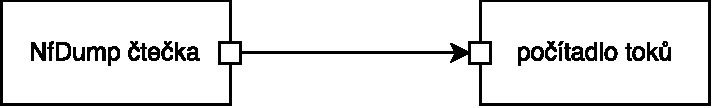
\includegraphics[width=0.5\textwidth]{fig/nemea-basic.pdf}
    \caption{Minimální příklad NEMEA systému obsahující pouze dva moduly.} \label{fig:nemea-schema}
  
\end{figure}

Z takto základních bloků lze postavit i velmi komplexní systém jak je vidět na obrázku \ref{fig:nemea-example-2}, kde jsou data přijímána v reálném čase z IPFIX\cite{ipfix} kolektoru. Data jsou předzpracována, analyzována několika algoritmy a následně jsou vytvořeny události, které jsou nahlášeny. Každá z těchto úloh je jeden modul, který může být znovu použitý na několika různých místech. Tím se šetří zdroje a nároky na tvorbu modulů.

\begin{figure}[h]
    \centering
    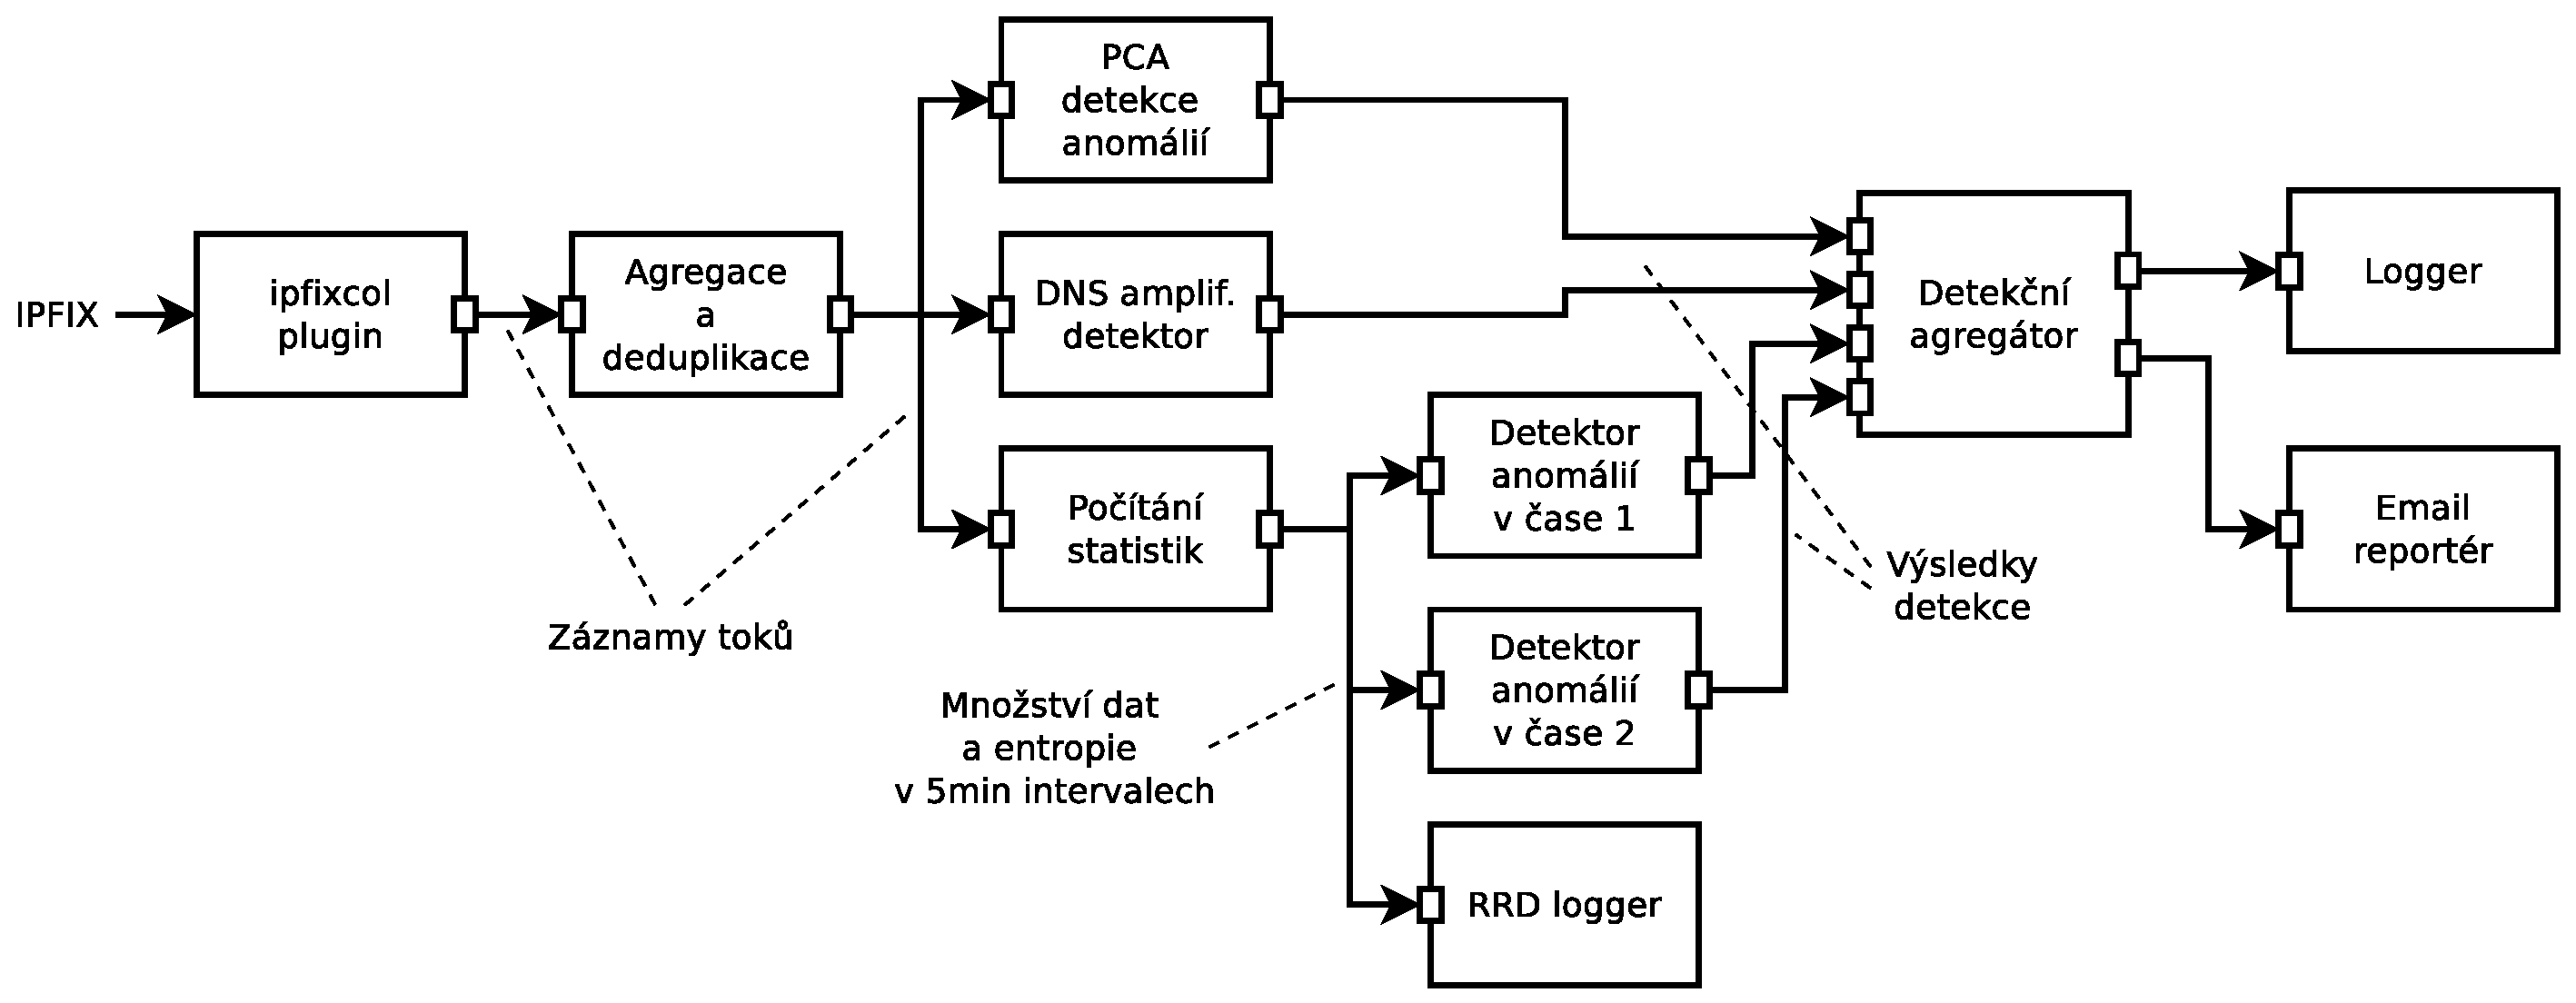
\includegraphics[width=1\textwidth]{fig/nemea-example-2-cz.eps}
    \caption{Komplexní příklad NEMEA systému, který kolektuje data, předzpracovává je, provádí detekci anomálií a útoků a následně detekované události ukládá a reportuje.} \label{fig:nemea-example-2}
  
\end{figure}


%\subsection*{Hlavní komponenty}

\subsection{Modul}

Každý modul je samostatný program nezávislý na ostatních. To sice zvyšuje nároky na systém, ale dovoluje větší variabilitu při návrhu modulu. Ten je, díky tomuto návrhu, možno naprogramovat v libovolném jazyce, sledovat a řídit spotřebu zdrojů každého modulu zvlášť a zejména v případě nefungujícího modulu se celý systém NEMEA dokáže zotavit z chyby naprosto bez problémů. Modulární systém navíc dovoluje přidávat a odebírat jednotlivé moduly za běhu, což je v produkčním prostředí jedna ze základních vlastnostní kvalitního monitorovacího systému.

Při zapojení a startu nového modulu se modul periodicky snaží připojit na definované rozhraní. Pokusy o spojení jsou sledovány NEMEA Supervisorem, kterým lze spravovat všechny moduly v systému a pokud se modulu nepodaří po několika pokusech připojit na rozhraní, je modul ukončen.

\subsection{Rozhraní}

Všechny rozhraní jsou výhradně jednocestná a přenos dat je realizován formou jednotlivých záznamů. Všechny záznamy poslané přes jedno konkrétní rozhraní mají vždy stejný formát, nicméně mezi rozhraními se formát může lišit. 

Protokol pro dynamickou tvorbu formátu je nazván UniRec. Ten specifikuje nejen formát záznamu, ale také jak záznam vytvořit a jak zpracovat -- implementuje formát pro binární reprezentaci síťového záznamu.

Pro tvorbu rozhraní je vytvořena sdílená knihovna libtrap, která využívá Traffic Analysis Platform (zkráceně TRAP) pro komunikaci mezi různými rozhranímia tyto rozhraní využívají protokolu UniRec.

\section{IDEA}
\label{sec:idea}

Pro potřebu sdílení informací o síťových událostech mezi různými skupinami a zařízeními (např. honeypoty, analyzéry systémových zpráv, analyzéry provozu na síti, netflow sondy a další) existuje několik formátů záznamu pro takovéto události. Nicméně žádný z nich není natolik univerzální, aby byl vždy a všude použitelný a pokud se k takovému formátu blíží, tak není natolik detailní, aby pokryl všechny důležité informace.

IDEA, neboli Intrusion Detection Extensible Alert, je formát záznamu síťové události specifikovaný sdružením CESNET. IDEA si klade za cíl specifikovat takový formát záznamu, který je univerzální, přenositelný, ale zároveň dost konkrétní a snadno pochopitelný bez potřeby rozsáhlé dokumentace k jednotlivým polím.

Vzorový záznam generovaný systémem NEMEA je vyobrazený ve výpisu \ref{code:idea}. Jak je vidět, formát je specifikovaný jako JSON dokument, aby byl přehledný, čitelný v běžné podobě (narozdíl od binárních formátů), lehce přenositelný a efektivní (např. oproti XML\cite{xmlvsjson}).

%\vspace{5mm}
\begin{figure}[h]
\lstset{basicstyle=\small,style=JSON}
\begin{lstlisting}
{
    "Format" :      "IDEA0",
    "ID" :          "73e0b136-aeb8-4aae-bb80-9bfb4f258847",
    "Category" :    ["Availibility.DDoS"],
    "Description" : "DNS amplification",
    "EventTime" :   "2016-04-07T22:19:25Z",
    "CreateTime" :  "2016-04-07T22:34:52Z",
    "CeaseTime" :   "2016-04-07T22:34:38Z",
    "DetectTime" :  "2016-04-07T22:34:38Z"
    "PacketCount" : 393,
    "Source" : [{
        "IP4" : ["192.1.0.201"],
        "Proto" : ["udp","dns"],
        "OutPacketCount" : 393,
        "InPacketCount" : 767
    }],
    "Target" : [{
        "Proto" : ["udp","dns"],
        "IP4" : ["10.0.0.135"],
        "InPacketCount" : 393
    }],
    "Node" : [{
        "SW" : ["NEMEA","amplification_detection"],
        "Name" : "cz.cesnet.nemea.amplification_detection"
    }],
    "Type" : ["Flow","Statistical"],
}
\end{lstlisting}
\captionof{lstlisting}{Vzorový IDEA záznam ze systému NEMEA. Některé části byly vynechány nebo zkráceny a IP adresy změněny na lokální.}
\label{code:idea}
\end{figure}

\newpage

\section{Další monitorovací systémy}

Na trhu jsou v současné době různá dostupná řešení pro detekci a vizualizaci síťových bezpečnostních událostí, nicméně valná hromada z nich je komerční a hlavně vázaná na konkrétní hardware od daného výrobce. Klient tudíž většinou nekupuje software, ale hardware s přiloženým software.

Komerčně dostupný produkt je např. Flowmon\cite{flowmon:report} ADS\cite{flowmon:ads} od stejnojmenné společnosti. Flowmon je spin-off společností z projektu Liberouter ze sdružení CESNET. Jejich sondy a kolektory využívají technologie vytvořené ve sdružení CESNET jak z hlediska hardware, tak software. Dalším komerčním řešením je Cisco Secure IDS\cite{cisco:ids}, dříve známý jako Cisco NetRanger.

Open source projekty jako NEMEA jsou dostupné mnoho let, ale pouze několik z nich dosáhlo znatelnějšího rozšíření v komunitě síťových správců. Nejvýznamnějšími jsou systémy Snort\cite{snort}, VERMONT\cite{vermont} a framework Bro\cite{bro}. 

\subsection*{Snort}
Tento open-source projekt, od roku 2013 vlastněn firmou Cisco\cite{snort:cisco}, je možno konfigurovat ve 3 hlavních režimech\cite{snort:modes}: \uv{sniffer}, paket logger a jako (N)IDS. V režimu IDS Snort pracuje principiálně velmi podobně jako systém NEMEA. Zachytává síťový provoz, ukládá si důležité informace o něm a analyzuje jej. Ve výsledku ukládá záznamy o síťových událostech. Nicméně Snort není modulárním systémem a tudíž není tak flexibilní a není stavěný na vysokorychlostní rozsáhlé sítě jako systém NEMEA.

\subsection*{VERMONT}

VERMONT (Versatile Monitoring Toolkit) je modulární monitorovací systém obsahující IPFIX kolektor, exportér, analyzátor a další moduly a grafické prostředí pro vizuální analýzu dat. VERMONT byl vyvinut v rámci projektu HISTORY\cite{vermont:history} a evropským projektem DIADEM firewall\cite{vermont:diadem}. Svou architekturou je nejbližší systému NEMEA, protože je částečně modulární. Systém NEMEA je oproti tomu modulární od samotného jádra systému, což dovoluje vyšší flexibilitu při vývoji a menší závislost na použitých technologií.

\subsection*{Bro}
Dalším v komunitě rozšířeným řešením je framework Bro. Tento framework primárně určený pro síťovou analýzu není podobný systému NEMEA, ani předchozím systémům, protože je to spíše nástroj pro vytváření (N)IDS než-li ucelený systém. Bro se velmi blíží skriptovacímu jazyku (např. Perl) nebo unixovým nástrojům jako tcpdump nebo nfdump. Bro lze rozdělit na dvě vrstvy. První vrstvou je \uv{Bro Event engine}, který analyzuje síťový provoz a generuje neutrální síťové události v podobě \uv{byla vytvořena nějaká událost}. 

Tyto neurčité události jsou následně analyzovány druhou vrstvou -- \uv{Bro Policy skripty}. V této vrstvě je naimplementovaný zmiňovaný skriptovací jazyk. V současné době existuje mnoho naprogramovaných skriptů, které jsou připraveny k okamžitému použití, včetně pokročilé analýzy síťového provozu.

V ranných fázích vývoje se systém NEMEA velmi blížil frameworku Bro, s vývojem času se ale NEMEA stala uceleným systémem připraveným k okamžitému nasazení na měřící body.

\section{Shrnutí}

V této kapitole jsme prezentovali systém NEMEA a jeho architekturu. Popsali jsme jeho nejdůležitější části, zejména jak vypadá modul a jeho komunikační protokol. Dále jsme popsali formát záznamu síťové bezpečnostní události IDEA, který je opěrným bodem pro ukládání dat v systému NEMEA v rámci analýzy událostí koncovým uživatelem. V poslední sekci jsme porovnali systém NEMEA s dalšími veřejně dostupnými monitorovacími systémy.

%%%%%%%%%%%%%%%%%%%%%%%%%%%%
% Kapitola 3
% Technologie
%%%%%%%%%%%%%%%%%%%%%%%%%%%%

\chapter{Technologie}

Vizualiace síťových bezpečnostních událostí může být vytvořena několika přístupy. Pokud máme IDS, který je dostupný pouze z jednoho stroje, nejčastěji zvolíme tvorbu desktopové aplikace, protože máme jistotu provozního prostředí. V případě vzdálené správy (častější případ) IDS jsme nejčastěji odkázání na vzdálený přístup pomocí příkazové řádky. Tento přístup je bohužel velmi limitovaný a nelze jej využít pro vizualiaci. V současné době je pro vzdálenou správu nejvhodnější vytvořit webovou aplikaci, která je dostupná z Internetu a použitelná na většině dnes používaných zařízeních\footnote{Jedná se zejména o stolní počítače, notebooky, tablety a chytré mobilní telefony.}

Pro tvorbu moderních webové aplikace (zkráceně MWA) je na Internetu dostupná celá řada knihoven, frameworků a systémů. Nicméně první otázkou zůstává co taková MWA je? 

Specifikem MWA je její vysoká interaktivita s uživatelem, vysoká dostupnost služby, kterou poskytuje a rozdělení na dva logické celky. Uživatelskou a serverovou část, často chybně nazývané frontend a backend aplikace. Více o architektuře aplikace v kapitole \ref{architektura}.

Vysoká interaktivita MWA je tvořena pomocí jazyka JavaScript. Ten umožňuje dynamickou změnu stránky bez nutnosti ji znova načítat a tím pádem uživatel nepřichází o dočasná data na stránce. Tento přístup navíc redukuje počet dotazů na server a snižuje tak jeho zátěž.

S přesunem logiky na uživatelskou část MWA jsou ale spojeny nemalé problémy. Zejména pak různorodá interpretace kódu. To se v posledních letech téměř eliminovalo díky moderním prohlížečům a jejich jádrům jako je např. WebKit pro Google Chrome nebo Gecko pro Firefox.

Často se MWA anglicky říká \uv{Single-page} aplikace\cite{spa}. Tento název je ale poněkud zavádějící. Povětšinou je aplikace natolik komplexní, že s jedinou stránkou bychom uživatele zmátli a přetížili informacemi a proto MWA strukturujeme do adresářové podoby. V tu chvíli již aplikace není jednostránková, ale vícestránková a název začíná být nepřesný.

\section{Dostupné technologie pro uživatelskou část}

K vytvoření MWA a zejména uživatelské části existuje několik významných systémů. V této části si tyto technologie představíme a porovnáme mezi sebou. Nejdůležitější částí je JavaScriptová knihovna/framework, který bude nejčastěji interagovat s uživatelem. Další nedílnou součástí je knihovna pro HTML/CSS, která bude definovat vzhled aplikace.

\subsection{JavaScript MVC frameworky}

Bylo vybráno 5 JavaScript MVC (Model-View-Controller)\cite{mvc} frameworků, které napomáhají k tvorbě MWA. Architektura MVC rozděluje aplikaci na tři celky, které mezi sebou navzájem komunikují. Více informací o MVC architektuře v kapitole \ref{architektura}.

Kritéria užšího výběru frameworků byla zejména následující:

\begin{itemize}  
\item open-source projekt s MIT nebo BSD licencí,
\item jednoduché použití,
\item nenáročný na výpočetní výkon hostitelského stroje,
\item široká podpora mezi prohlížeči,
\item projekt má určitou historii a je udržován některou ze známých společností (udržitelnost vývoje).
\end{itemize}

\subsubsection*{React\cite{react}}
Framework React je vyvíjen pod hlavičkou společnosti Facebook. Původním cílem návrhářů Reactu bylo vyřešit problémy během vývoje komplexních uživatelských rozhraní s rychle měnícími se daty. Dalším cílem bylo vytvořit takový framework, který lze distribuovat v takovém měřítku jako je Facebook.

React je framework pro uživatelskou část MWA používající tradiční MVC architekturu. Taková architektura je nejvíce znatelná v případě použití obousměrného vázání dat (anglicky two-way data binding), více v sekci \ref{sec:mvc}.

React se zaměřuje zejména na tvorbu UI, z pohledu architektury pohledová část (view), a kvůli tomu se ostatním částem architektury nevěnuje tak detailně, jak by většinu času vývojář potřeboval. Velmi častým řešením je použít React na pohledovou část a na model a kontrolér použít jiný framework, např. AngularJS.

Z této pozice se React nadále vyvíjí 

React pracuje s moderními přístupy k vývoji MWA a boří tak mnoho zažitých technik jak MWA vyvíjet. Místo běžné manipulace s DOM elementy si React, případně vývojář, definuje vlastní DOM elementy, kterým přídává určité vlastnosti, váže na ně data a pohodlně s nimi manipuluje bez větších výkonových ztrát. Toho docílil zejména použitím tzv. shadow DOM\cite{shadowdom}, který je ale novinkou na poli prohlížečů a je podporován pouze jádrem WebKit. Pokud ale není shadow DOM dostupný, používá React standardní DOM, se kterým je sice vykreslování pomalejší, ale stále velmi rychlé. 

\begin{figure}[ht]
\lstset{basicstyle=\small,style=JSON}
\begin{lstlisting}
var HelloMessage = React.createClass({
    render: function() {
        return <div>Hello {this.props.name}</div>;
    }
});

ReactDOM.render(<HelloMessage name="John" />, mountNode);
\end{lstlisting}
\captionof{lstlisting}{\uv{Hello World} příklad v jazyku JSX, který do stránky vykreslí text \uv{Hello John}.}
\label{code:react}
\end{figure}

Pro názornou ukázku, jak framework React funguje, je ve výpise \ref{code:react} vytvořen jednoduchý \uv{Hello World} element v JSX\cite{jsx} syntaxi. Tento kód demonstruje pouze minimální možnosti frameworku, ale vypovídá o jednoduchosti použití Reactu.

\subsubsection*{Ember.js}

Ember.js je primárně zaměřen na tvorbu SPA. Toho dosahuje zejména používáním zažitých praktik v rámci komunity vývojářů, širokou funkcionalitou bez nutnosti instalace dalších doplňků a osvědčil se i vysokou stabilitou během celé doby vývoje. Ember je také vždy jedním z prvních frameworků, který implementuje novinky obsažené v nových jádrech webových prohlížečů jako jsou např. JavaScript Promises\cite{jspromises}, Web Components\cite{webcomponents} nebo ES6 syntaxe.

Ember se skládá celkem z pěti klíčových konceptů. Jejich názvy jsou ponechány anglicky pro větší názornost.

\begin{itemize}  
    \item {\bf Routes} -- každý stav aplikace je reprezentován unikátní cestou a této cestě náleží i odpovídající objekt, který manipuluje s danou cestou.
    \item {\bf Models} -- každá cesta má svůj korespondující model, který obsahuje data asociována s danou cestou a stavem aplikace. Model slouží zejména k manipulaci s daty.
    \item {\bf Templates} -- šablony jsou tvořeny v HTML s použitím šablonovacího jazyka HTMLBars\cite{htmlbars}.
    \item {\bf Components} -- komponenta je vlastní HTML značka definovaná programátorem aplikace. Její chování je implementováno pomocí JavaScriptu a její vzhled pomocí HTMLBars šablon. Komponenta se chová jako běžný DOM element.
    \item {\bf Services} -- servis je singleton objekt, který v sobě udržuje dlouhodobá data během používání aplikace klientem.
\end{itemize}

\subsubsection*{Backbone.js}

Framework Backbone se mírně odlišuje od předešlých frameworků a to zejména architekturou, která není MVC, ale MVP (model-view-presenter).

\subsubsection*{AngularJS}

Framework AngularJS je jedním z nejdéle existujících frameworků pro tvorbu MWA.

\subsubsection*{Polymer}

\subsection*{HTML/CSS knihovny}
\subsubsection*{Bootstrap}
\subsubsection*{Angular Material}
\subsubsection*{Foundation}

\subsection{Serverová část}
\subsubsection*{Python Flask}
\subsubsection*{PHP}
\subsubsection*{C++ a Mongoose}
\subsubsection*{NodeJS}





\section{Výběr technologií}
\subsection{Uživatelská část}

\subsection{Serverová část}

\section{Zvolené technologie}

\chapter{Architektura aplikace}
\label{architektura}

\begin{figure}[h]
    \centering
    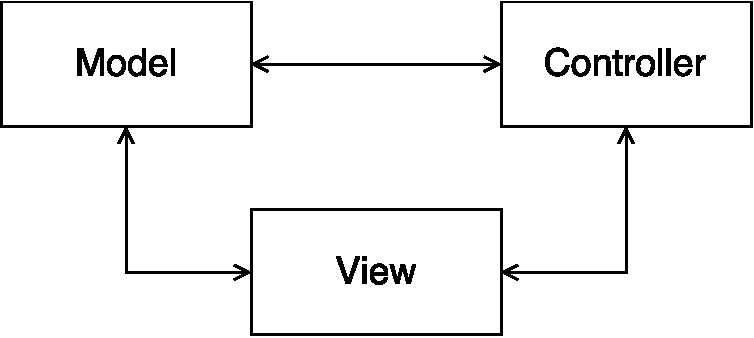
\includegraphics[width=0.5\textwidth]{fig/mvc.pdf}
    \caption{MVC architektura} \label{fig:mvc}
  
\end{figure}

\section{MVC}
\label{sec:mvc}


\section{Případy užití}
\section{REST API}
\section{Databáze událostí}
\section{GUI}

\chapter{Implementace}
\section{Backend}
\section{Frontend}
\section{Zabezpečení}
\section{Distribuce}

\chapter{Dosažené výsledky}
\section{Názory uživatelů}
\section{Nasazení v praxi}

\chapter{Závěr}
Závěrečná kapitola obsahuje zhodnocení dosažených výsledků se zvlášť vyznačeným vlastním přínosem studenta. Povinně se zde objeví i zhodnocení z pohledu dalšího vývoje projektu, student uvede náměty vycházející ze zkušeností s řešeným projektem a uvede rovněž návaznosti na právě dokončené projekty.

%=========================================================================
 % viz. obsah.tex

  % Pouzita literatura
  % ----------------------------------------------
\ifslovak
  \makeatletter
  \def\@openbib@code{\addcontentsline{toc}{chapter}{Literatúra}}
  \makeatother
  \bibliographystyle{czechiso}
\else
  \ifczech
    \makeatletter
    \def\@openbib@code{\addcontentsline{toc}{chapter}{Literatura}}
    \makeatother
    \bibliographystyle{czechiso}
  \else 
    \makeatletter
    \def\@openbib@code{\addcontentsline{toc}{chapter}{Bibliography}}
    \makeatother
    \bibliographystyle{plain}
  %  \bibliographystyle{alpha}
  \fi
\fi
  \begin{flushleft}
  \bibliography{literatura} % viz. literatura.bib
  \end{flushleft}

  % Prilohy
  % ---------------------------------------------
  \appendix
\ifczech
  \renewcommand{\appendixpagename}{Přílohy}
  \renewcommand{\appendixtocname}{Přílohy}
  \renewcommand{\appendixname}{Příloha}
\fi
\ifslovak
  \renewcommand{\appendixpagename}{Prílohy}
  \renewcommand{\appendixtocname}{Prílohy}
  \renewcommand{\appendixname}{Príloha}
\fi
  \appendixpage

\ifslovak
  \section*{Zoznam príloh}
  \addcontentsline{toc}{section}{Zoznam príloh}
\else
  \ifczech
    \section*{Seznam příloh}
    \addcontentsline{toc}{section}{Seznam příloh}
  \else
    \section*{List of Appendices}
    \addcontentsline{toc}{section}{List of Appendices}
  \fi
\fi
  \startcontents[chapters]
  \printcontents[chapters]{l}{0}{\setcounter{tocdepth}{2}}
  \chapter{Vzorový IDEA záznam}
\label{code:idea}

\begin{figure}[ht]
\lstset{basicstyle=\small,style=JSON}
\begin{lstlisting}
{
    "Format" :      "IDEA0",
    "ID" :          "73e0b136-aeb8-4aae-bb80-9bfb4f258847",
    "Category" :    ["Availibility.DDoS"],
    "Description" : "DNS amplification",
    "EventTime" :   "2016-04-07T22:19:25Z",
    "CreateTime" :  "2016-04-07T22:34:52Z",
    "CeaseTime" :   "2016-04-07T22:34:38Z",
    "DetectTime" :  "2016-04-07T22:34:38Z"
    "PacketCount" : 393,
    "Source" : [{
        "IP4" : ["192.1.0.201"],
        "Proto" : ["udp","dns"],
        "OutPacketCount" : 393,
        "InPacketCount" : 767
    }],
    "Target" : [{
        "Proto" : ["udp","dns"],
        "IP4" : ["10.0.0.135"],
        "InPacketCount" : 393
    }],
    "Node" : [{
        "SW" : ["NEMEA","amplification_detection"],
        "Name" : "cz.cesnet.nemea.amplification_detection"
    }],
    "Type" : ["Flow","Statistical"],
}
\end{lstlisting}
\captionof{lstlisting}{Vzorový IDEA záznam ze systému NEMEA. Některé části byly vynechány nebo zkráceny a IP adresy anonymizovány.}
\end{figure}


\chapter{Drátěné modely aplikace}

\begin{figure}[ht]
    \centering
    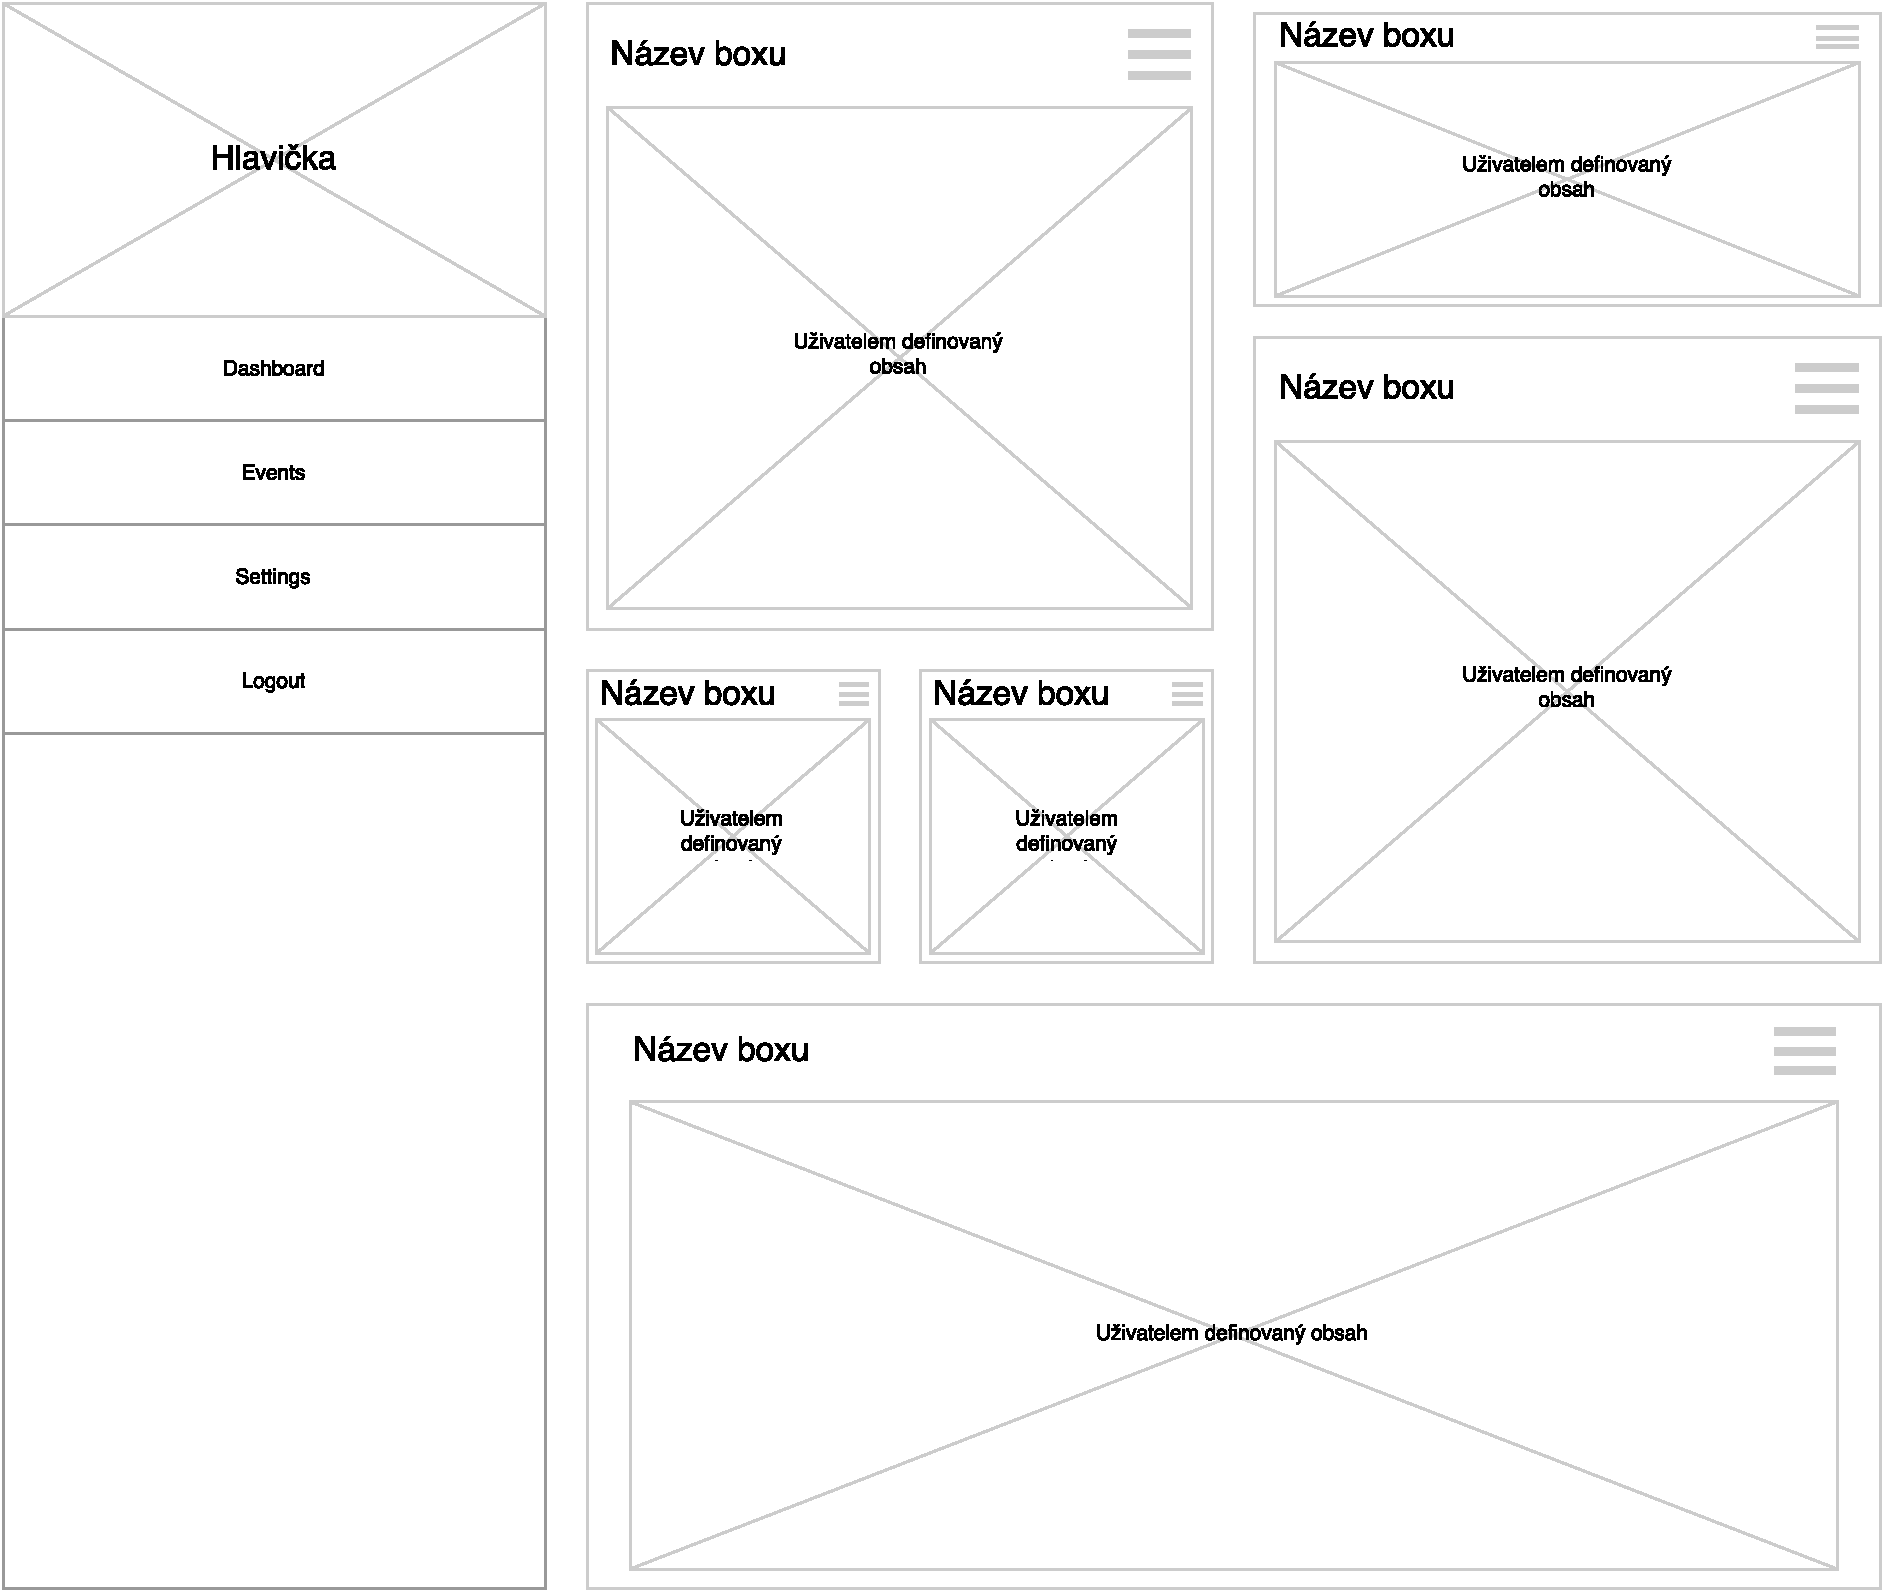
\includegraphics[width=1\textwidth]{fig/wf_dashboard.pdf}
    \caption{Drátěný model pro dashboard, který uživatel může konfigurovat.} \label{wf:dashboard}
\end{figure}

\begin{figure}[ht]
    \centering
    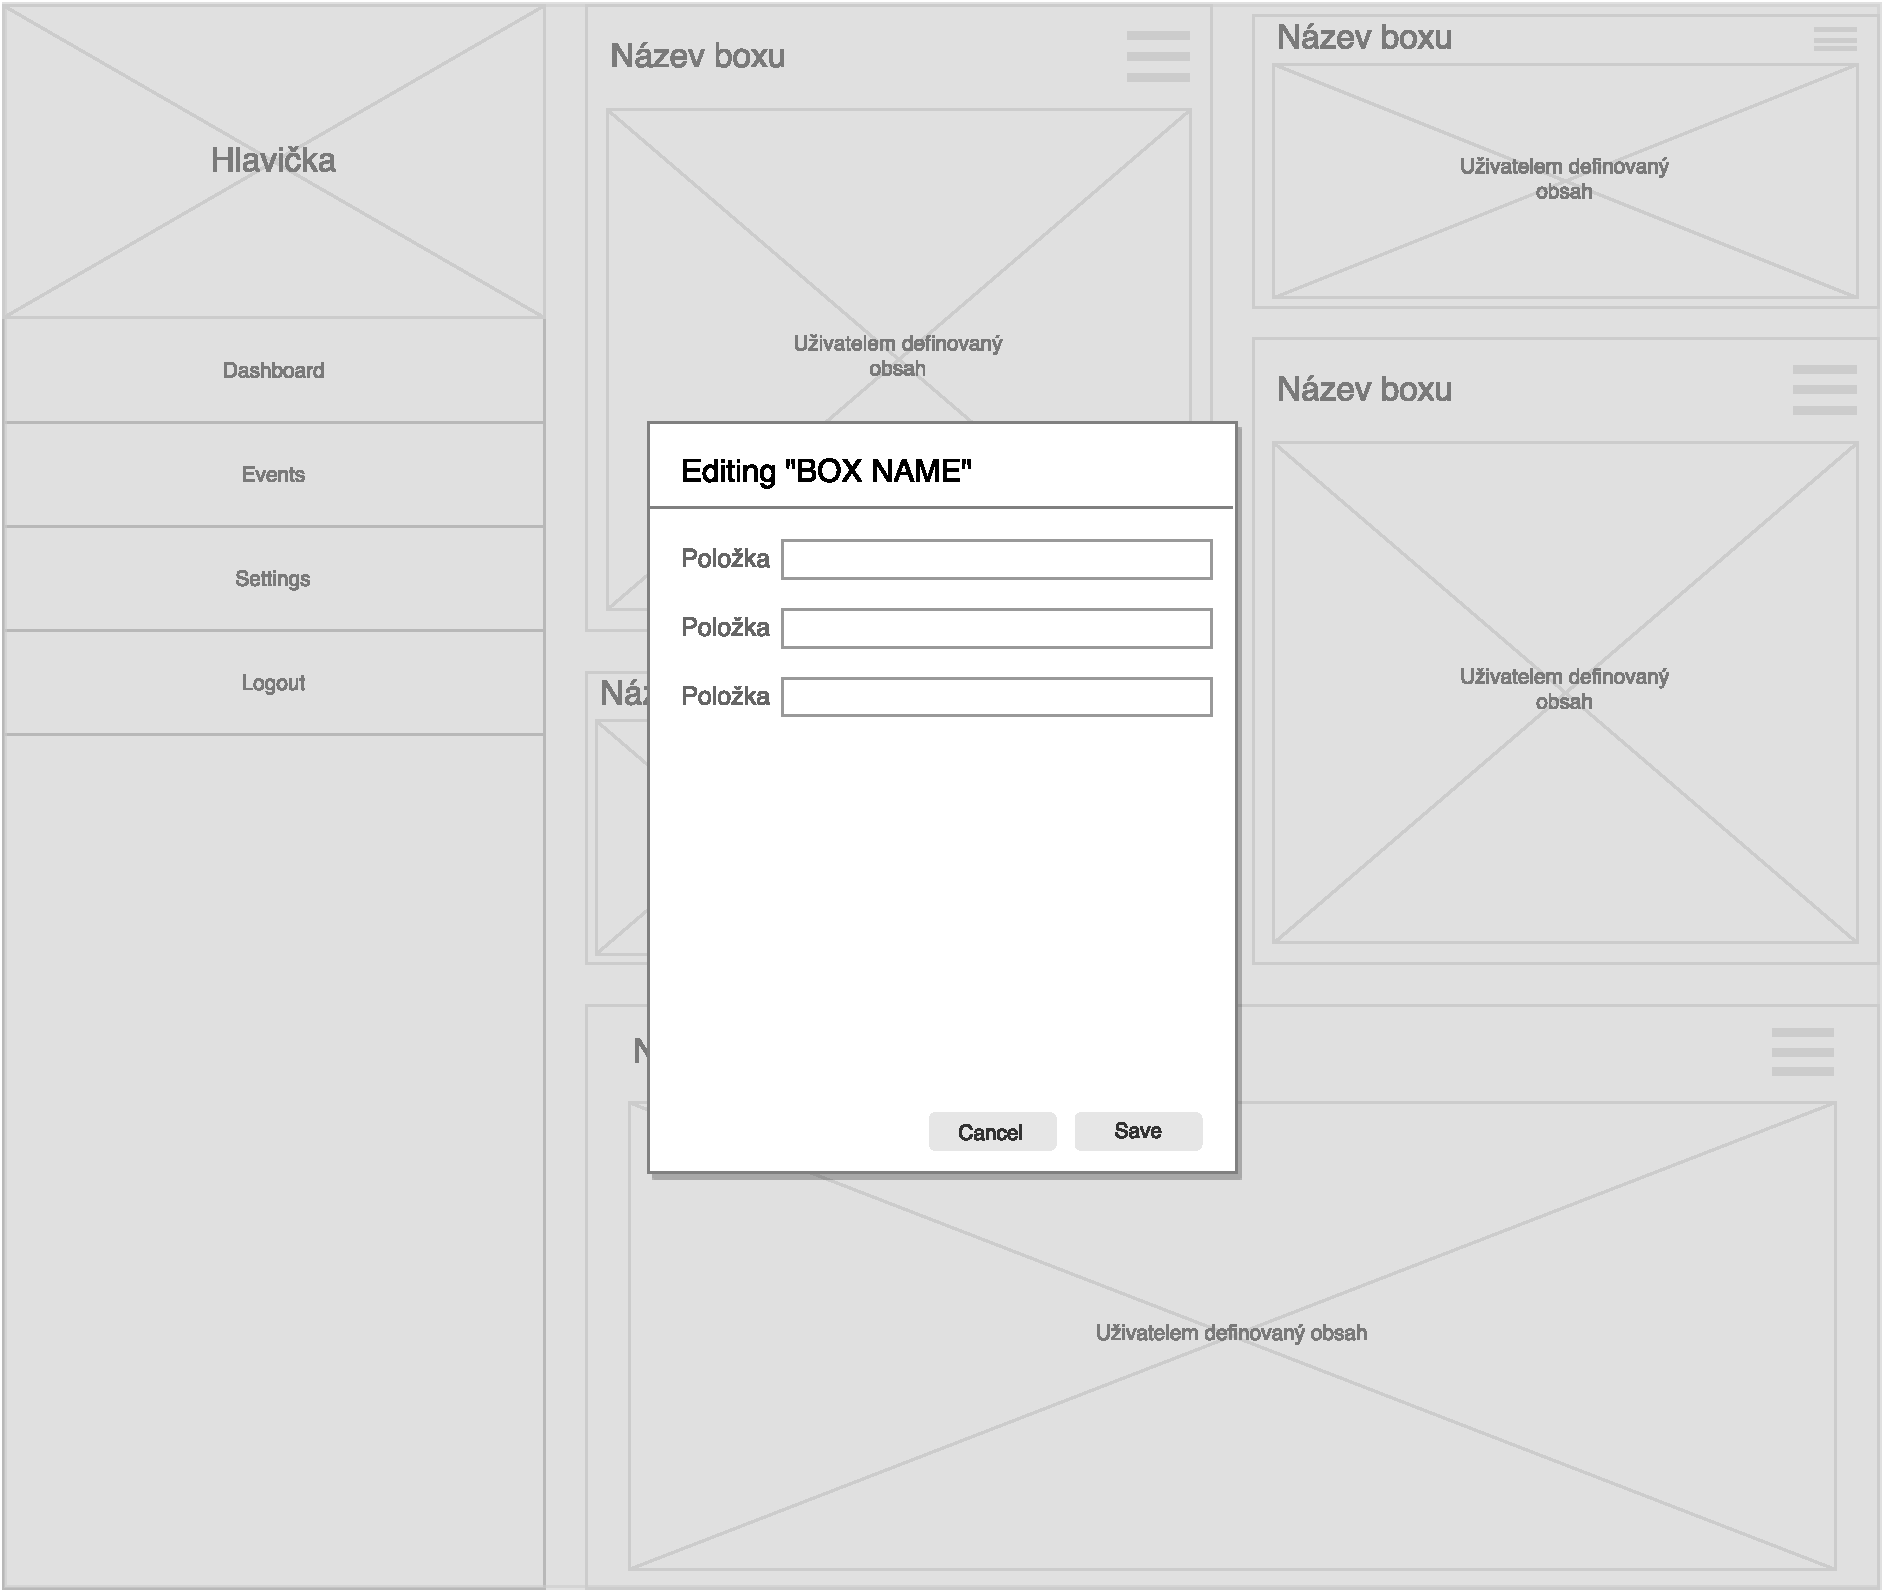
\includegraphics[width=1\textwidth]{fig/wf_dashboard_edit.pdf}
    \caption{Konfigurace boxu v dashboardu.} \label{wf:dashboard_edit}
\end{figure}


\begin{figure}[ht]
    \centering
    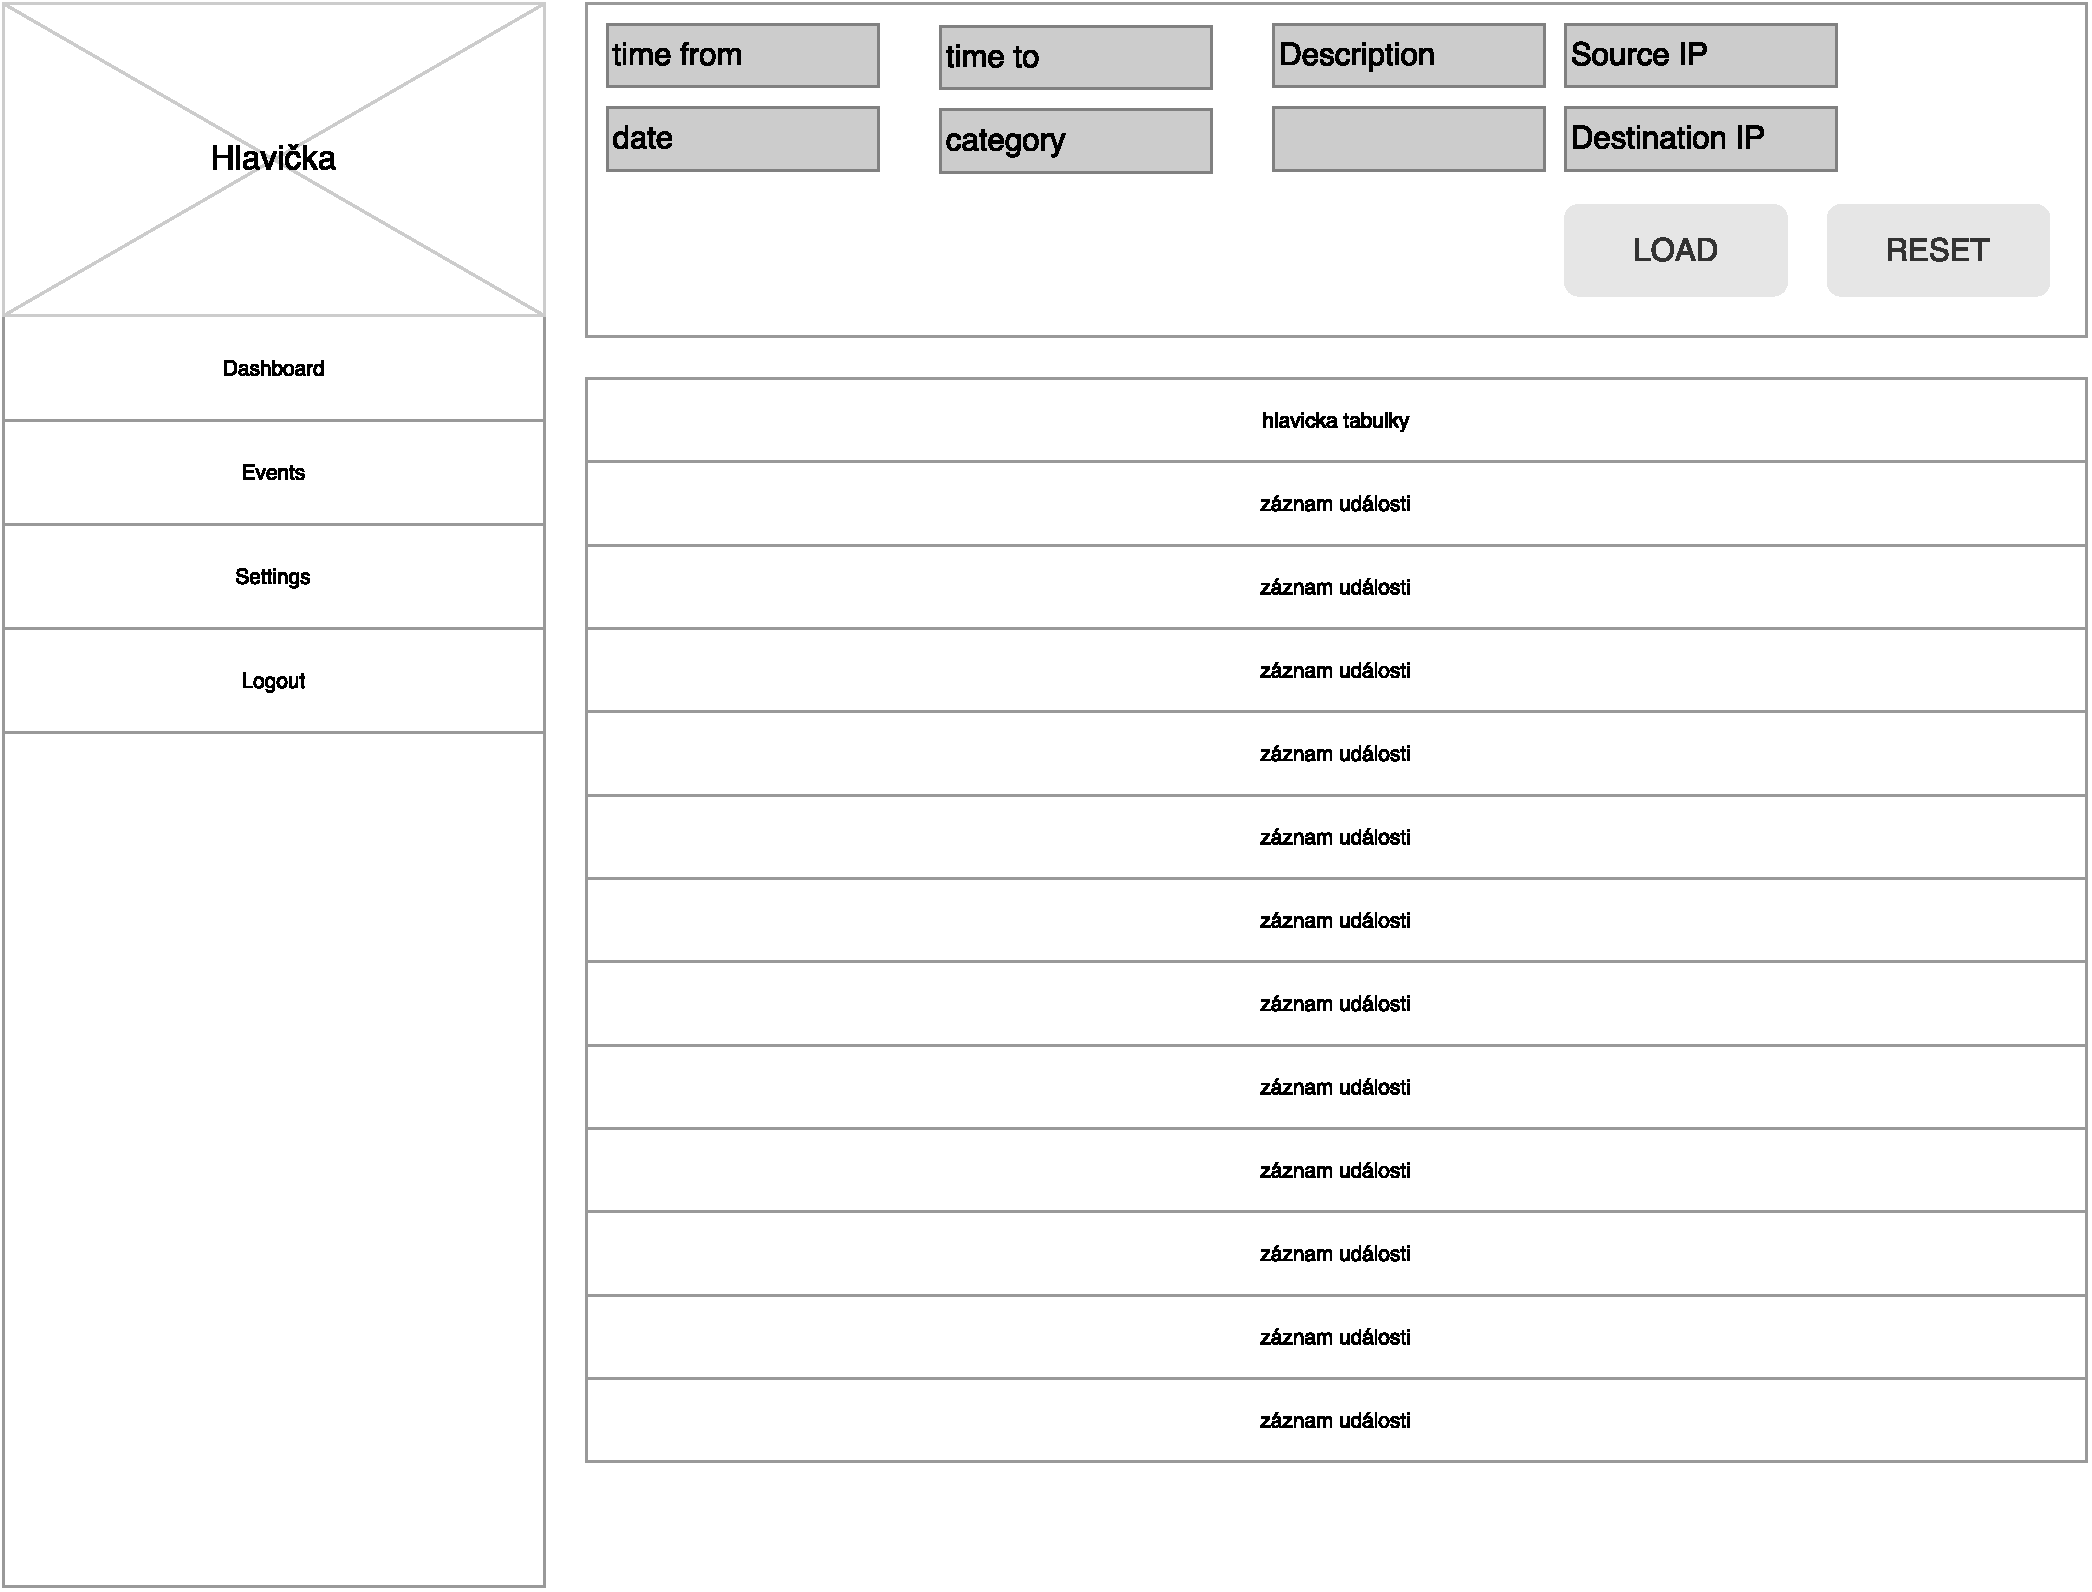
\includegraphics[width=1\textwidth]{fig/wf_dashboard_events.pdf}
    \caption{Přehled vyfiltrovaných událostí.} \label{wf:dashboard_events}
\end{figure}

\chapter{Seznam použitých Python knihoven}

\begin{figure}[ht]
\lstset{basicstyle=\small,style=JSON}
\begin{lstlisting}
Flask==0.10.1
Flask-Cors==2.1.2
itsdangerous==0.24
Jinja2==2.8
MarkupSafe==0.23
py-bcrypt==0.4
pycparser==2.14
PyJWT==1.4.0
pymongo==3.2
six==1.10.0
Werkzeug==0.11.3
\end{lstlisting}
\captionof{lstlisting}{Obsah souboru requirements.txt, který využívá nástroj pip pro instalaci Python knihoven.}
\label{code:requirements}
\end{figure}

\chapter{Snímky uživatelské strany před akceptačními testy}
\label{screens:before}

\begin{figure}[ht]
    \centering
    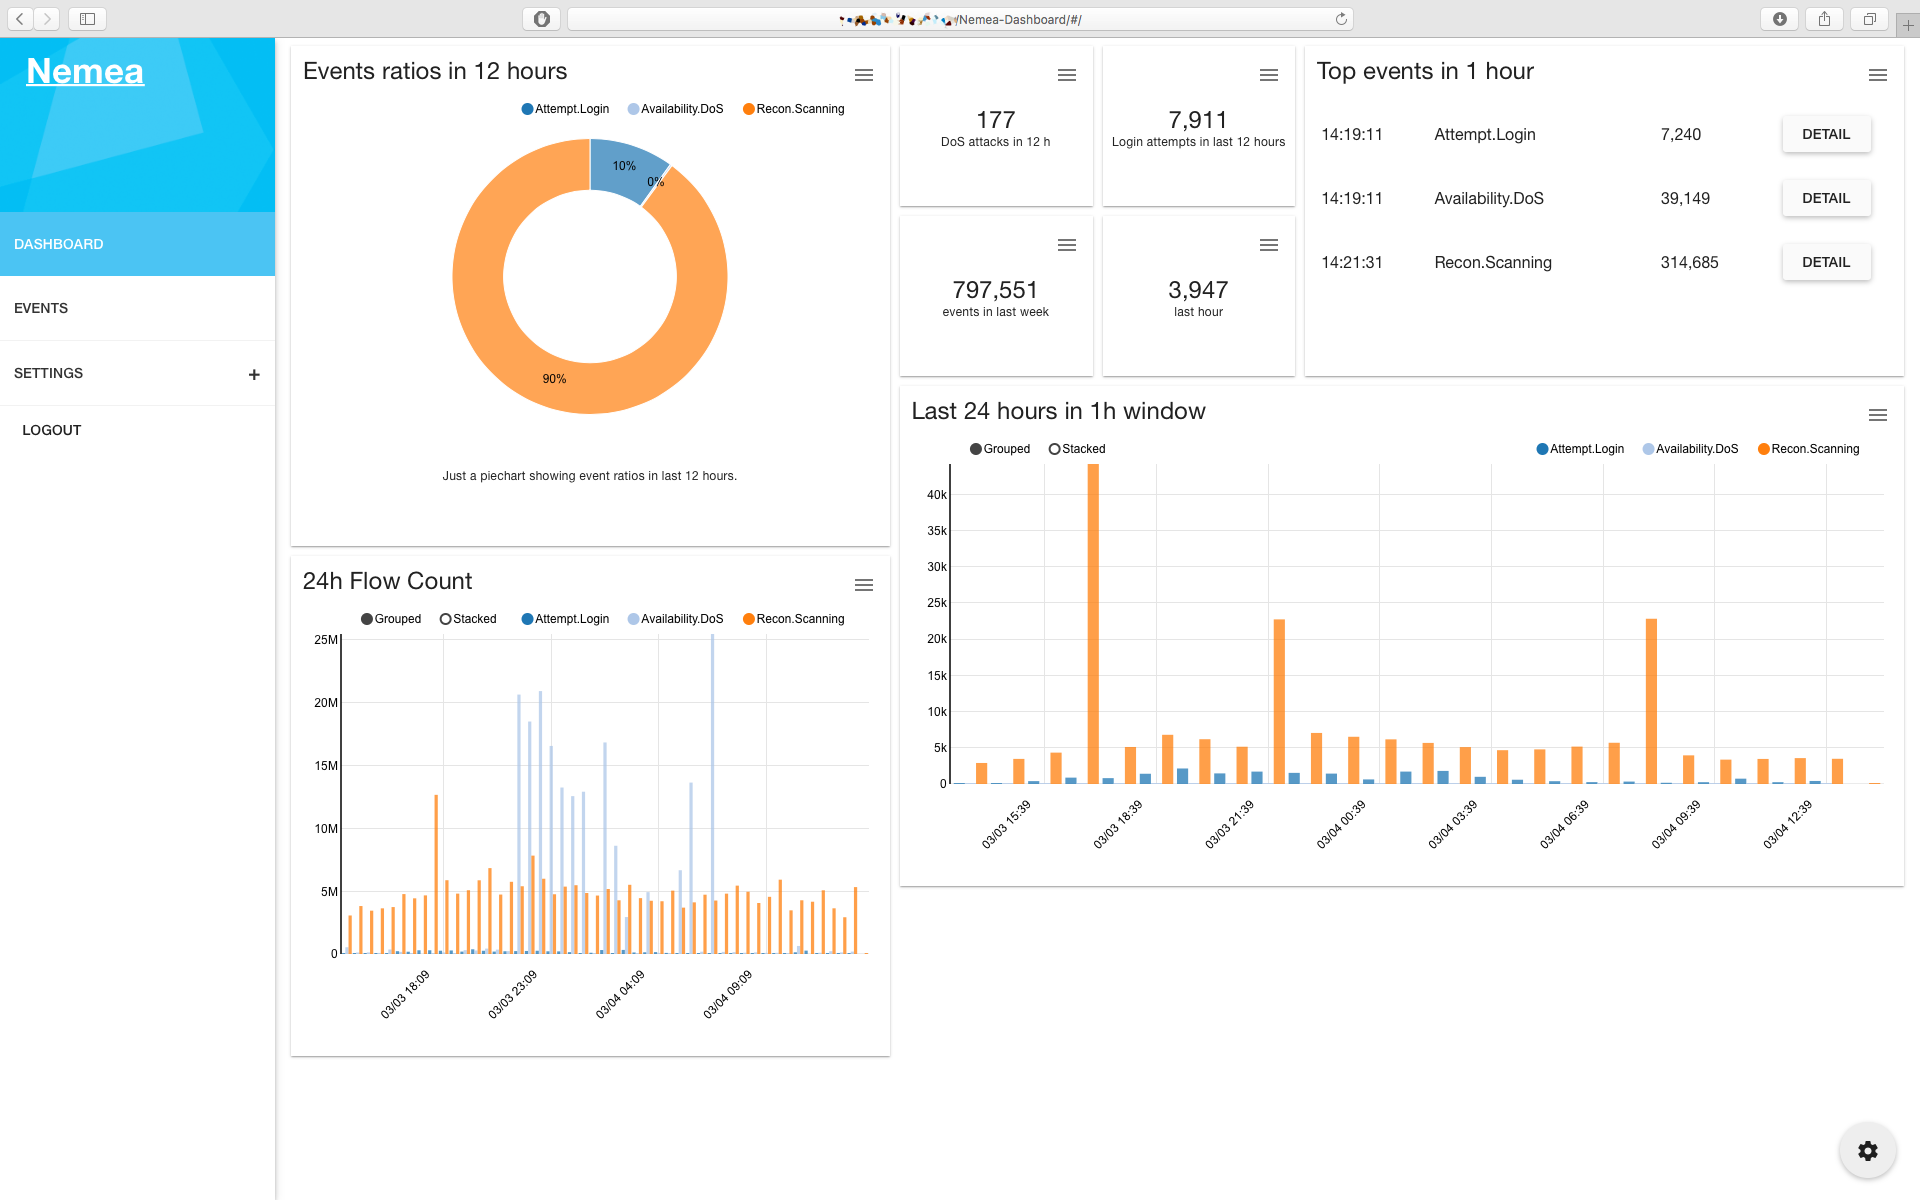
\includegraphics[width=1\textwidth]{fig/screen_before_1.png}
    \caption{Úvodní obrazovka s přednastavenými boxy.} \label{screen:before:1}
\end{figure}

\begin{figure}[ht]
    \centering
    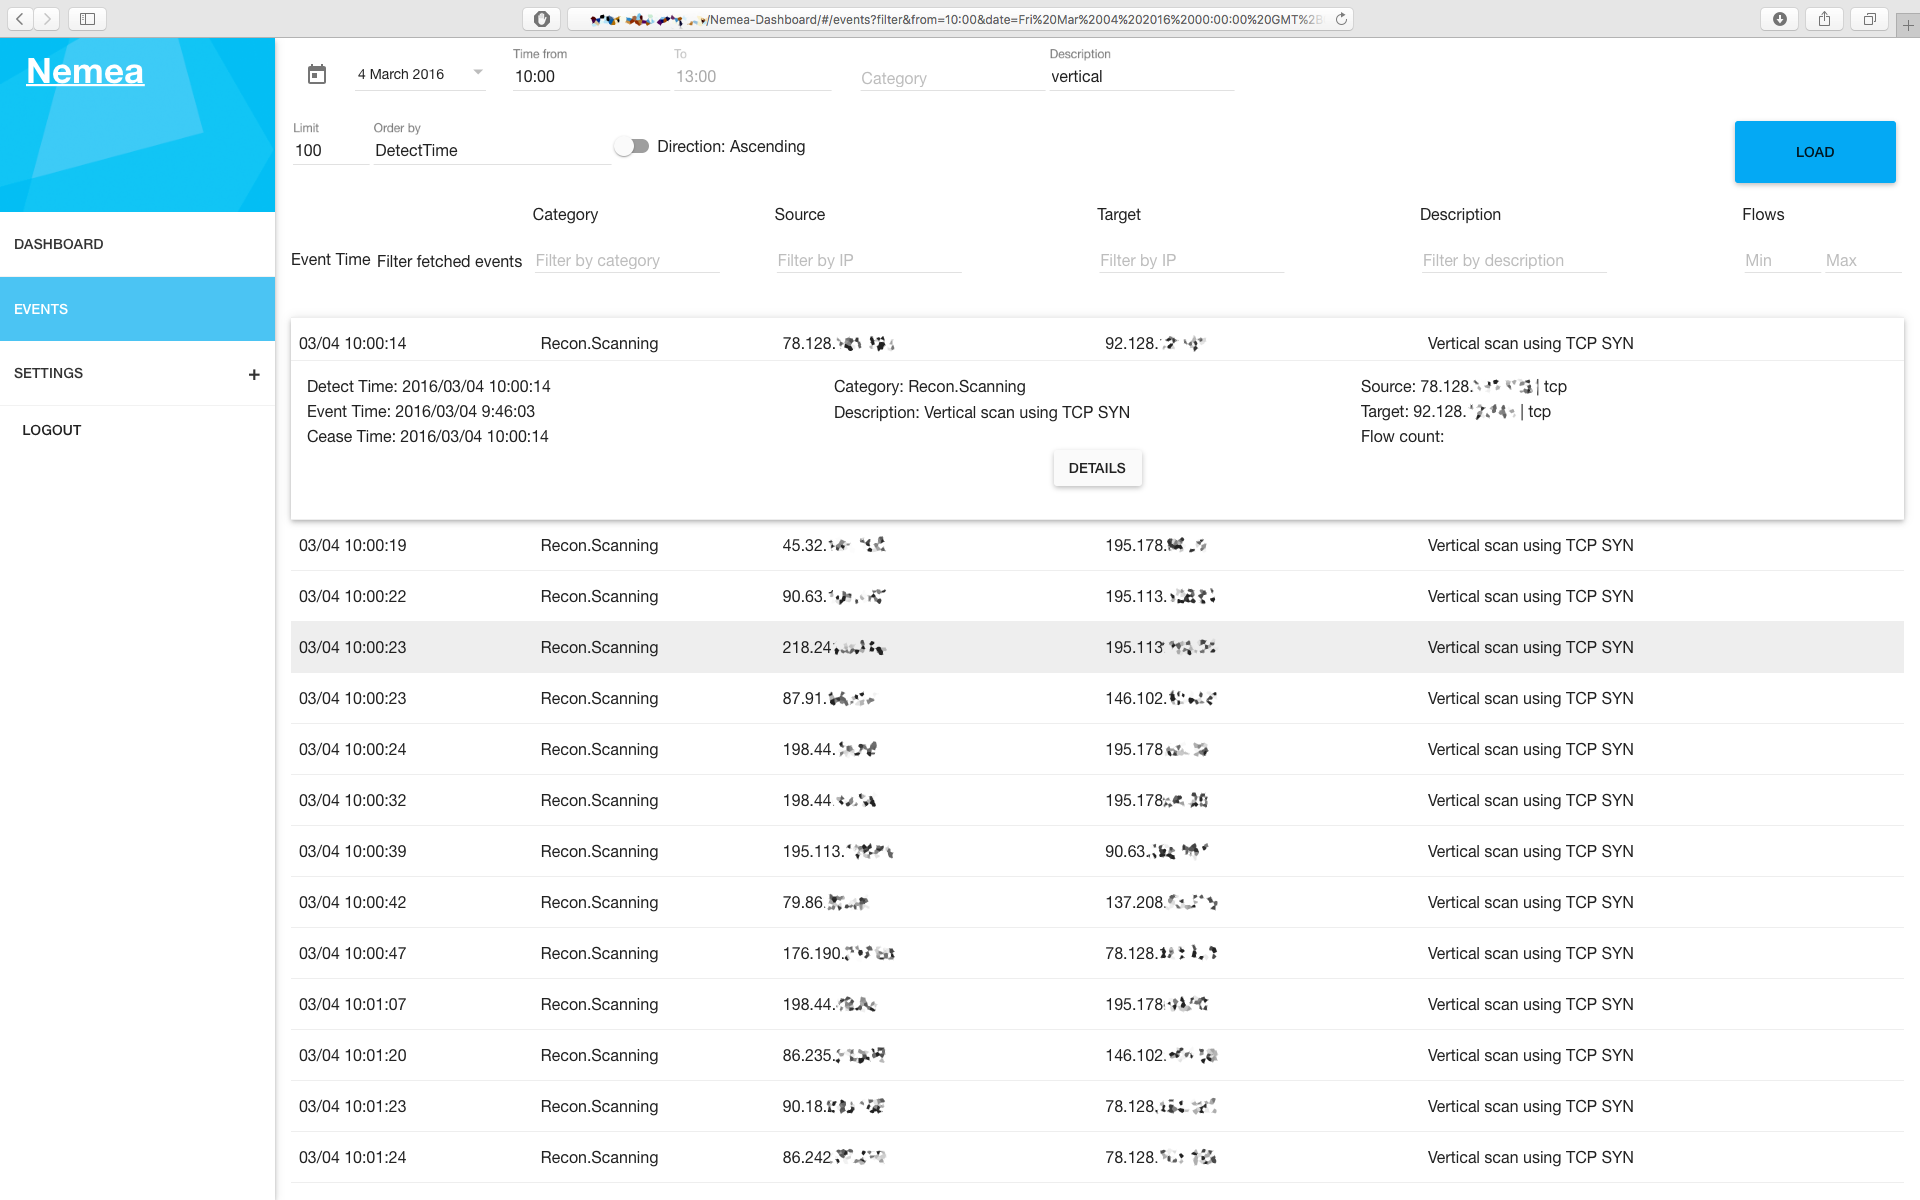
\includegraphics[width=1\textwidth]{fig/screen_before_2.png}
    \caption{Výpis nalezených událostí.} \label{screen:before:2}
\end{figure}

\begin{figure}[ht]
    \centering
    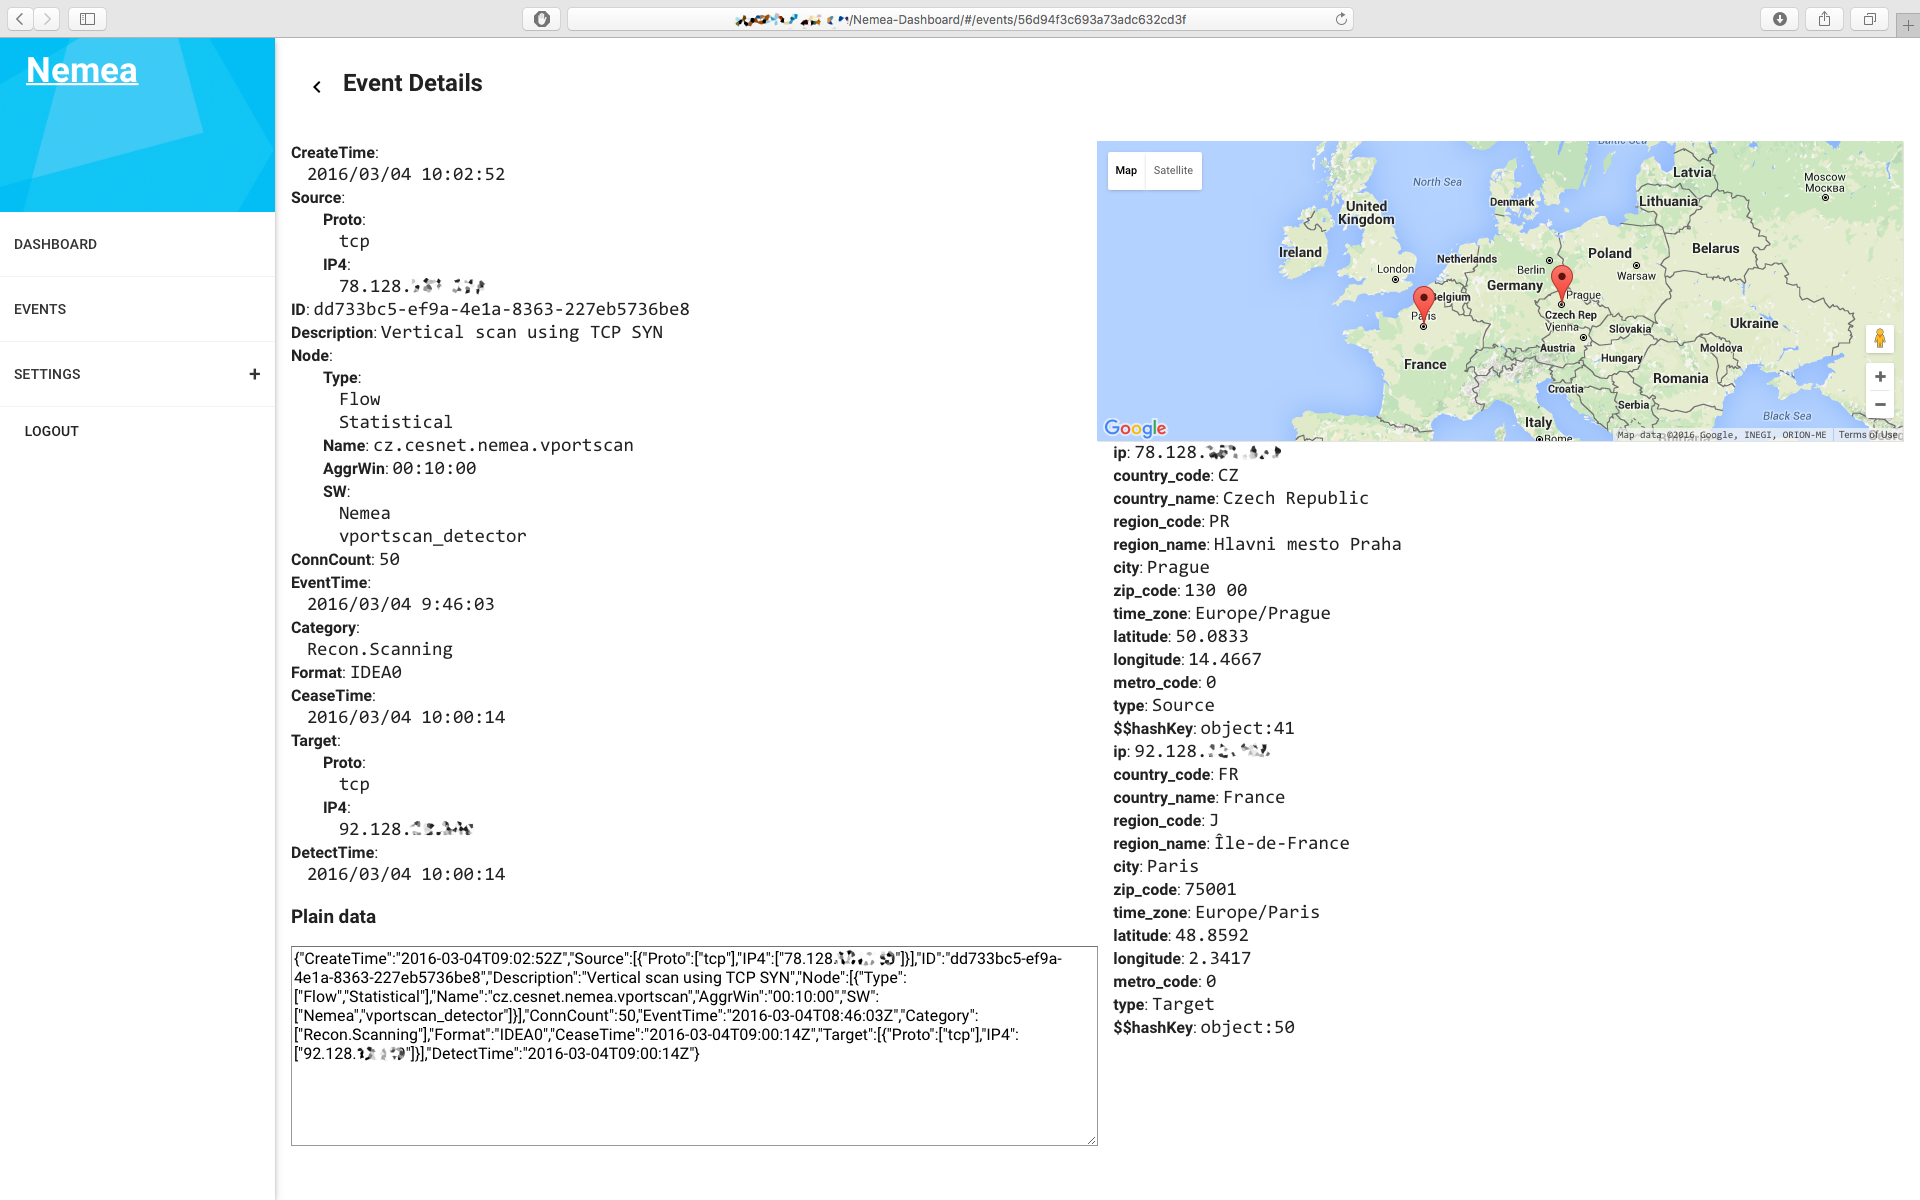
\includegraphics[width=1\textwidth]{fig/screen_before_3.png}
    \caption{Detail události.} \label{screen:before:3}
\end{figure}



\chapter{Snímky uživatelské strany po prvním kole testů}
\label{screens:after}

\begin{figure}[ht]
    \centering
    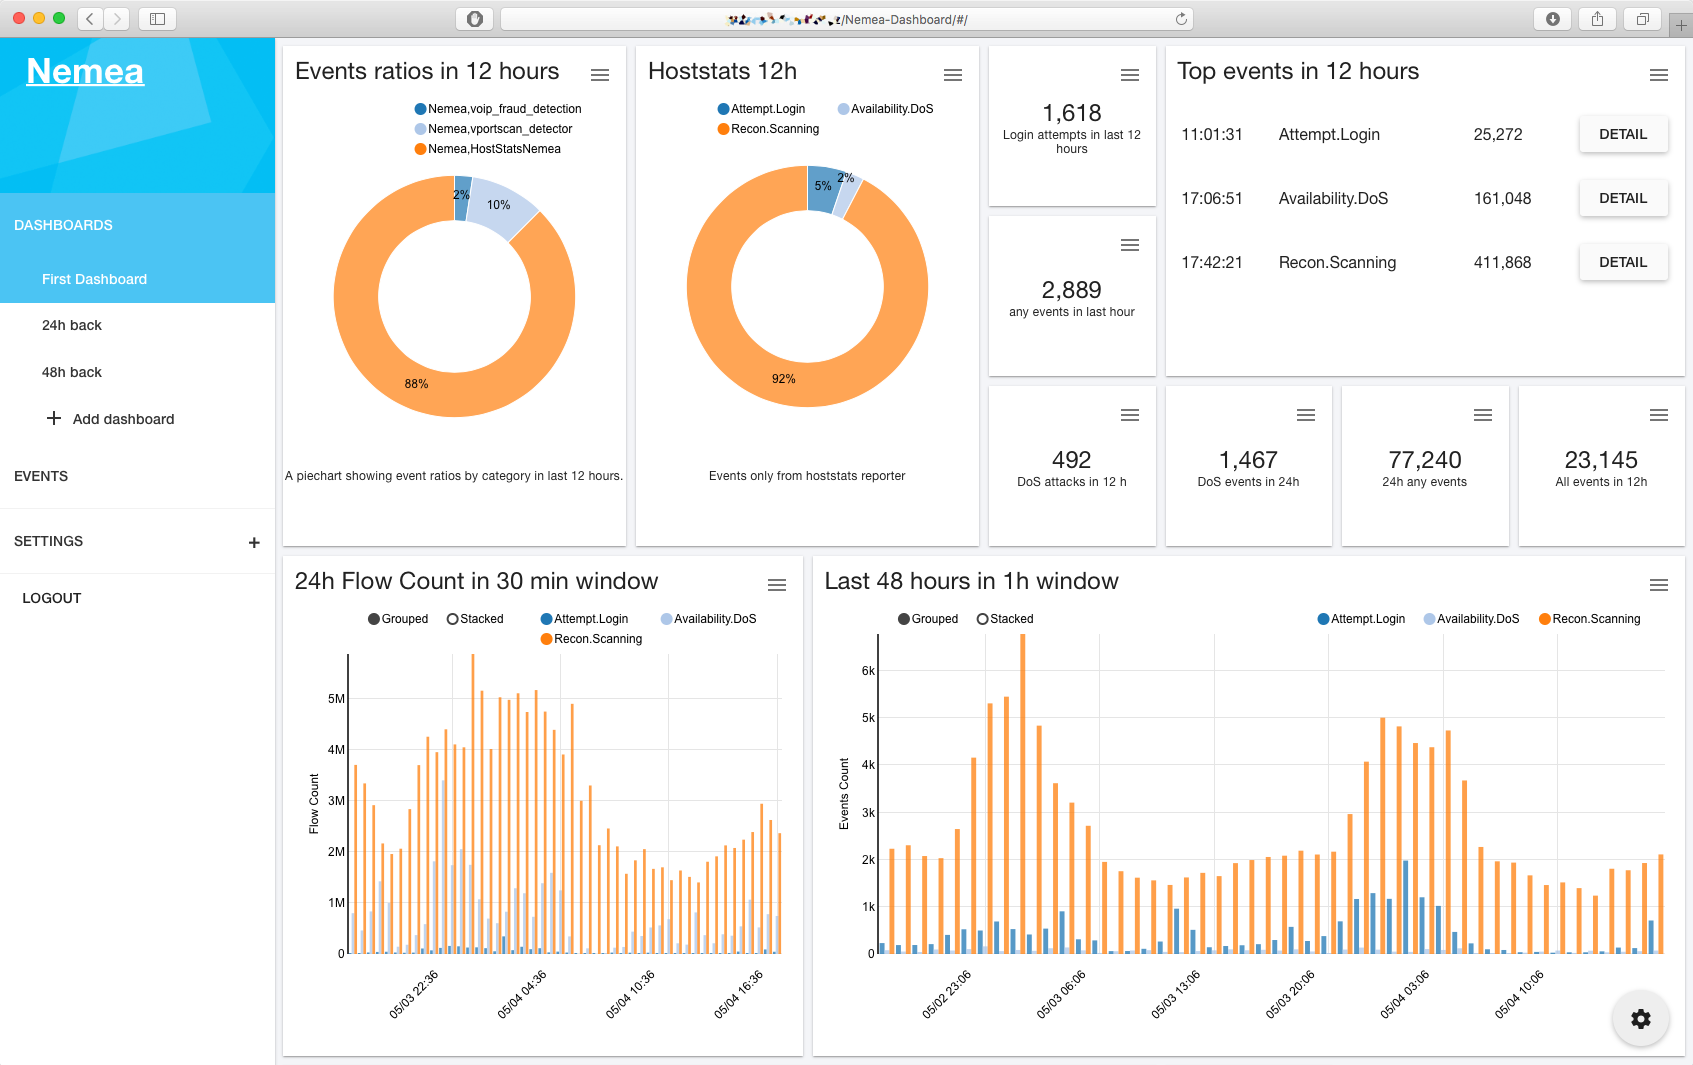
\includegraphics[width=1\textwidth]{fig/screen_after_1.png}
    \caption{Úvodní obrazovka s přednastavenými boxy.} \label{screen:after:1}
\end{figure}

\begin{figure}[ht]
    \centering
    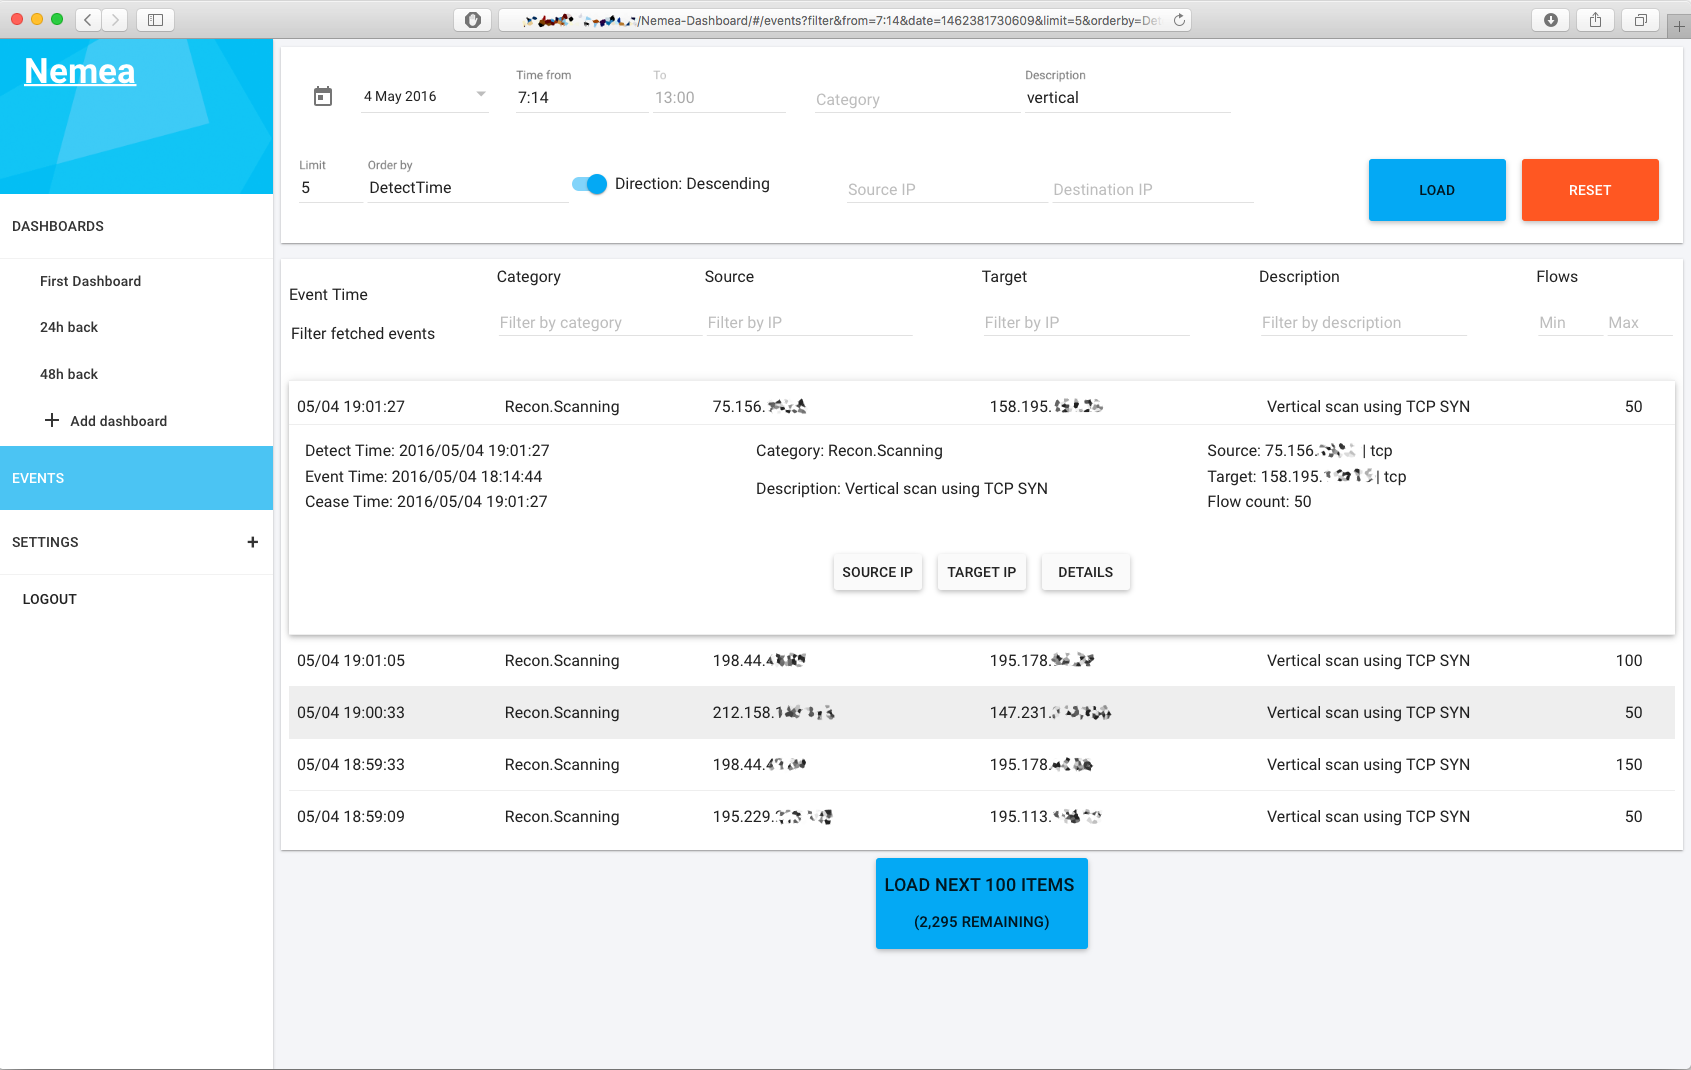
\includegraphics[width=1\textwidth]{fig/screen_after_2.png}
    \caption{Výpis nalezených událostí.} \label{screen:after:2}
\end{figure}

\begin{figure}[ht]
    \centering
    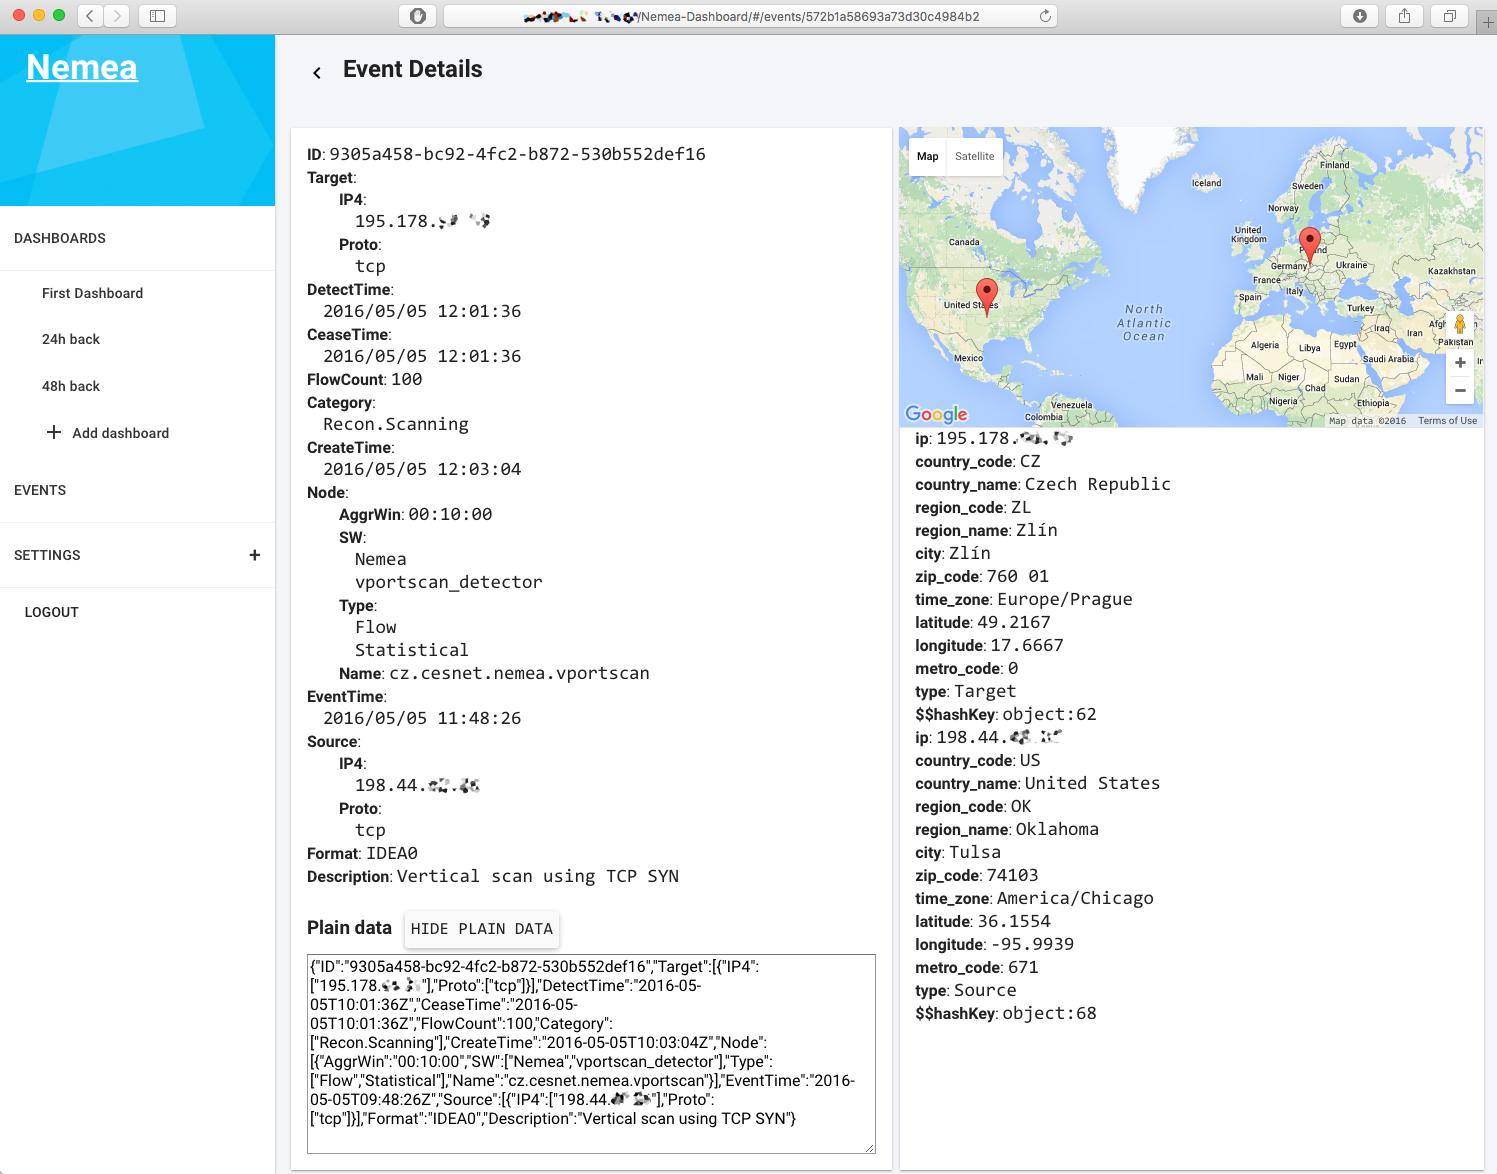
\includegraphics[width=1\textwidth]{fig/screen_after_3.png}
    \caption{Detail události.} \label{screen:after:3}
\end{figure}



\chapter{Obsah DVD}
%\chapter{Manual}
%\chapter{Konfigrační soubor}
%\chapter{RelaxNG Schéma konfiguračního soboru}
%\chapter{Plakat}

 % viz. prilohy.tex
\end{document}
